\documentclass[sn-mathphys,Numbered]{sn-jnl}% Math and Physical Sciences Reference Style
%\documentclass[sn-mathphys,Numbered,draft]{sn-jnl}% Math and Physical Sciences Reference Style

%%\documentclass[sn-nature]{sn-jnl}% Style for submissions to Nature Portfolio journals
%%\documentclass[sn-basic]{sn-jnl}% Basic Springer Nature Reference Style/Chemistry Reference Style
%%\documentclass[sn-aps]{sn-jnl}% American Physical Society (APS) Reference Style
%%\documentclass[sn-vancouver,Numbered]{sn-jnl}% Vancouver Reference Style
%%\documentclass[sn-apa]{sn-jnl}% APA Reference Style 
%%\documentclass[sn-chicago]{sn-jnl}% Chicago-based Humanities Reference Style
%%\documentclass[default]{sn-jnl}% Default
%%\documentclass[default,iicol]{sn-jnl}% Default with double column layout

%%%% Standard Packages
%%<additional latex packages, if required can be included here>

\setlength{\parskip}{\baselineskip}

\usepackage{graphicx}%
\usepackage{amsmath,amssymb,amsfonts,bm}%
\usepackage{multirow}
\usepackage{amsthm}%
%\usepackage{subcaption}
\usepackage{mathrsfs}%
\usepackage[title]{appendix}%
\usepackage{xcolor}%
\usepackage{textcomp}%
\usepackage{manyfoot}%
\usepackage{booktabs}%
%\usepackage{algorithm}%
%\usepackage{algorithmicx}%
\usepackage{algpseudocode}%
\usepackage{listings}%
\usepackage{bigints}
\usepackage{outlines}
\usepackage{geometry}
\usepackage{subfigure}
\usepackage{siunitx}
\usepackage{float}
\usepackage{comment}

\geometry
{
a4paper,         % or letterpaper
textwidth=15cm,  % llncs has 12.2cm
textheight=24cm, % llncs has 19.3cm
% heightrounded,   % integer number of lines
% hratio=1:1,      % horizontally centered
% vratio=2:3,      % not vertically centered
}
\setlength{\tabcolsep}{0.5cm}
\usepackage[onehalfspacing]{setspace}
% \usepackage{lineno}
% \linenumbers
%%%%

\usepackage[utf8]{inputenc}
\usepackage{graphicx}
\usepackage[ruled,vlined]{algorithm2e}
\usepackage{amsmath}
%\usepackage{movie15} %to allow movie embedding
\usepackage{enumitem}
\usepackage{color,soul}
\usepackage{xfrac}

%% New math commands
\newcommand{\s}[1]{\overset{*}{#1}}
\newcommand{\RM}{\bm{\Lambda}}
\newcommand{\RMI}{\bm{\Lambda}_0}
\newcommand{\RMT}{\bm{\Lambda}_t}
\newcommand{\RV}{\bm{\psi}}
\newcommand{\magRV}{\psi}
\newcommand{\RMTS}{\s{\bm{\Lambda}}_t}
\newcommand{\bb}{\boldsymbol}
\usepackage{nicefrac}
%\usepackage{tikz}
%\usepackage{tikz-3dplot}
\usepackage{mathtools}

%% For contact
\newcommand{\rbar}{\bar{\bm{r}}}
\newcommand{\xibar}{\bar{\xi}}
%\newcommand{\magRV}{\bbit{\psi}}
\newcommand{\diag}{\rm diag}


\begin{document}

\title[Article Title]{A Jacobian-free Newton-Krylov method for cell-centred finite volume solid mechanics}

\author[1,2]{\fnm{Ivan} \sur{Batisti\'{c}}}
\author[1,3]{\fnm{Pablo} \sur{Castrillo}}
\author*[1]{\fnm{Philip} \sur{Cardiff}}\email{philip.cardiff@ucd.ie}

\affil*[1]{\orgdiv{School of Mechanical and Materials Engineering}, \orgname{University College Dublin}, \orgaddress{\country{Ireland}}}
\affil[2]{\orgdiv{Faculty of Mechanical Engineering and Naval Architecture}, \orgname{University of Zagreb}, \orgaddress{\country{Croatia}}}
\affil[3]{\orgdiv{Instituto de Estructuras y Transporte, Facultad de Ingeniería}, \orgname{Universidad de la República}, \orgaddress{\country{Uruguay}}}

\abstract
{
%\coffeestainA{0.2}{0.85}{-25}{5cm}{10.3cm}
This work extends the application of Jacobian-free Newton–Krylov (JFNK) methods to higher-order cell-centred finite-volume formulations for solid mechanics.
While conventional cell-centred schemes are typically restricted to second-order accuracy, we present third- and fourth-order formulations that employ local least-squares reconstructions for gradient evaluation combined with Gaussian quadrature at cell faces for flux integration.
These schemes enable accurate resolution of complex stress and deformation fields in both linear and nonlinear solid mechanics, while retaining the flexibility and geometric generality of finite-volume methods.
A novel contribution of this study is the development and assessment of a JFNK solution strategy for these higher-order formulations, which eliminates the need to assemble and store large Jacobian matrices explicitly.
Instead, we demonstrate that a compact-stencil approximate Jacobian can be effectively employed as a preconditioner, mirroring the efficiency gains observed in second-order frameworks.
The proposed methodology is benchmarked across a suite of two- and three-dimensional test problems involving elastic and nonlinear materials, where key performance metrics, including accuracy, computational cost, memory usage, and robustness, are systematically evaluated.
Results confirm that the higher-order formulations deliver substantial accuracy improvements over second-order schemes, while the JFNK approach achieves strong performance and scalability with only minimal modifications to existing segregated frameworks.
These findings underscore the potential of combining higher-order finite-volume methods with JFNK solvers to advance the state of the art in computational solid mechanics.
The implementations are openly released in the solids4foam toolbox for OpenFOAM, supporting further exploration and adoption by the community.
}



\keywords{Jacobian-free Newton-Krylov, higher-order, cell-centred finite volume method, GMRES, solids4foam, OpenFOAM}

\maketitle


%%%%%%%%%%%%%%%%%%%%%%%%%%%%%%%%%%%%%%%%%%%%%%%%%%%%%%%%%%%%%%%%%%
\section{Introduction}\label{sec:intro}
%%%%%%%%%%%%%%%%%%%%%%%%%%%%%%%%%%%%%%%%%%%%%%%%%%%%%%%%%%%%%%%%%%
%Paper outline:
%
%Intro
Potential structure of this section:

	1.	Higher-order discretisation in computational solid mechanics remains relatively underexplored compared to fluid dynamics, despite its potential for improving accuracy and efficiency. Comment on 'why' we should care about higher order: potentially cheaper to achieve the same mesh error; potential to reduce the amount of data when running large models on HPC systems (where data is the bottleneck).

	2.	Recent research has demonstrated that higher-order accuracy can be achieved in cell-centred formulations through gradient reconstruction (e.g. least-squares approaches) and face integration techniques (e.g. Gaussian quadrature); however, their efficiency and ease of implementation in an industrial code are unexplored.

	3.	The solution strategy is a crucial factor: segregated iterative solvers remain the standard in finite-volume solid mechanics but often suffer from slow convergence and limited robustness, and they are efficient for higher orders, as shown by Demirdzic.
	Jacobian-free Newton–Krylov (JFNK) methods have emerged as a promising alternative, avoiding the need for explicit Jacobian construction while enabling quadratic convergence through Krylov subspace acceleration.
	In addition, the JFNK approach is well-suited for integration into existing segregated frameworks.

	4.	Our previous work established the feasibility and efficiency of JFNK for second-order cell-centred formulations, where a compact-stencil approximate Jacobian proved highly effective as a preconditioner.
	This study extends JFNK to third- and fourth-order cell-centred finite-volume formulations for linear and nonlinear solid mechanics, combining least-squares gradient reconstruction with Gaussian quadrature integration.

	5.	We demonstrate that the proposed approach significantly improves accuracy while retaining computational efficiency, and we show that compact-stencil Jacobians remain effective as preconditioners in the higher-order setting.

	6.	The aim of this paper is therefore twofold: to contribute to the relatively sparse literature on higher-order cell-centred finite-volume methods for solids, and to explore the synergy between such methods and Jacobian-free Newton–Krylov solution strategies.
	
	7. pokazano je da se moze splitat surface topologija cv-a na surface
	skica molekule na symmetry planeu
skica molekule na dirichlet boundariu
sve jedna slika na kojoj je desni rub dirichlet, dole je symmetry a gore je neumman rub!

Philip comment: we should mention the importance of using consistent areas and
volumes, e.g when discretising the volumetric terms we should use the same cell
decomposition as we use to calculate the cell volume; the same applies for the
face area integrals. Ivan noted this is required for non-flat faces to get the
expected order of accuracy, e.g. on the irregular hexahedra/polyhedra meshes.

%
%%%%%%%%%%%%%%%%%%%%%%%%%%%%%%%%%%%%%%%%%%%%%%%%%%%%%%%%%%%%%%%%%%%%%%%%%%%%%%%
%      
\section{Mathematical Model}
\label{sec:math_model}
%
%%%%%%%%%%%%%%%%%%%%%%%%%%%%%%%%%%%%%%%%%%%%%%%%%%%%%%%%%%%%%%%%%%%%%%%%%%%%%%%
%
For arbitrary body of volume $\Omega$ bounded by surface $\Gamma$ with outward facing unit normal $\bb{n}$
the strong integral form of linear momentum in \emph{total} Lagrangian form is:
%
\begin{eqnarray} \label{eqn:momentum_TL}
     \int_{\Omega_o} \rho_o \frac{\partial^2 \bb{u} }{\partial t^2} \text{d}\Omega_o
     =
     \oint_{\Gamma_o} \left( \bb{n}_o \cdot  \bb{P}^T\right)  \text{d}\Gamma_o
     + \int_{\Omega_o}  \bb{f}_b \, \text{d}\Omega_o,
\end{eqnarray}
%
where $\rho$ is density, $\bb{u}$ is the displacement vector, $\bb{P}$ is the first Piola–Kirchhoff stress tensor,
and $\bb{f}_b$ is a body force per unit volume, e.g., $\rho \bb{g}$, where $\bb{g}$ is gravity.
Subscript $o$ is used to indicate quantities in the initial reference configuration.
Through Nanson's formula it is possible to relate the first Piola–Kirchhoff stress tensor with the Cauchy $\bb{\sigma}$ stress tensor in the current configuration:
%
\begin{equation} \label{eqn:nanson}
\bb{P}=J \bb{\sigma} \bb{F}^{-\text{T}},
\end{equation} 
%
where $\bb{F}$ is deformation gradient defined as $\textbf{I} + (\bb{\nabla}_o \bb{u})^{\text{T}}$ and $J$ is its determinant $J = \text{det}(\bb{F})$.
\\
This work also considers linear geometry formulation, i.e. small strain assumption:
%
\begin{eqnarray} \label{eqn:momentum_lingeom}
    \int_{\Omega} \rho \frac{\partial^2 \bb{u} }{\partial t^2} \, \text{d}\Omega
     =
     \oint_{\Gamma} \bb{n} \cdot \bb{\sigma}_s \,  \text{d}\Gamma
     + \int_{\Omega}  \bb{f}_b \, \text{d}\Omega,
\end{eqnarray}
%
where $\bb{\sigma}_s$ is the engineering (small strain) stress tensor which coincide with Piola stress tensor.

Constitutive relation for Cauchy $\bb{\sigma}$ stress in Equations \ref{eqn:nanson} and \ref{eqn:momentum_lingeom} is given by a chosen mechanical law. 
Mechanical laws considered in this work (Hooke's law, St.\,Venant-Kirchhoff, Mooney–Rivlin, neo-Hookean, and Guccione) are briefly outlined in Appendix \ref{app:mechLaws}.
The governing equations are complemented by boundary conditions, with three types considered here: prescribed displacement, prescribed traction, and symmetry.
%
%%%%%%%%%%%%%%%%%%%%%%%%%%%%%%%%%%%%%%%%%%%%%%%%%%%%%%%%%%%%%%%%%%%%%%%%%%%%%%%
%      
\section{High-order Finite Volume Discretisation}
\label{sec:math_model}
%
%%%%%%%%%%%%%%%%%%%%%%%%%%%%%%%%%%%%%%%%%%%%%%%%%%%%%%%%%%%%%%%%%%%%%%%%%%%%%%%
%
In this work, a finite volume discretization is employed to approximate the strong form of the governing equations. 
The computational points are located at the cell centroids, where the solution is treated as point-valued rather than cell-averaged. 
This type of discretization is commonly referred to as the deconvolution finite volume method \cite{Nishikawa2025, Nishikawa2021}.

The spatial domain is partitioned into a finite set of contiguous convex polyhedral control volumes, each denoted by $P$.
Representative control volumes in 2D and 3D settings is is shown in Figure \ref{fig:cell}. 
The computational node associated with each cell $P$ is positioned at the cell centroid $\bb{x}_P$, the cell volume is denoted by $\Omega_P$,
and the centroid of a neighboring control volume is denoted by $N$.
Each control volume is bounded by a set of polygonal faces, which are categorized as follows:
\begin{itemize}
\item[•] Internal faces — shared between adjacent control volumes. The centroid of an internal face is denoted by $f$, its outward unit normal vector by $\bb{n}_f$, and its face area by $\Gamma_f$.
\item[• ] Boundary faces — located on the boundary of the spatial domain. The centroid of a boundary face is denoted by $b$, its outward unit normal vector by $\bb{n}_b$, and its surface area by $\Gamma_b$. 
\end{itemize}
%a face center 𝐱jk of a quadrilateral face between the cells 𝑗 and 𝑘 can be defined by the arithmetic average
%Estimating the residual requires calculating the volume integral of the source term
%129 and the surface integral of the normal flux for each cell. This is achieved using Gaussian
%130 integration, where a weighted sum of values at quadrature points is used to approximate
%131 the integral. The source integral calculation is performed as a weighted sum of values of
%132 the source term at the interior quadrature points for each cell. The flux integral part
%133 requires estimating the normal flux at quadrature points along the boundary of each cell
%Napisati da 2d probleme tretiramo kao 2D, nije standardni openfoam pristup - hibridna je kombinacija
%
%------------------------------------------------------------------------------
%\subsection{Solution domain discretisation}
%------------------------------------------------------------------------------
%
% The volume of an internal finite volume Ω𝑣
%is denoted as 𝑉𝑣 and the area of a face Σ𝑓 is denoted as 𝐴𝑓. The out-
%ward normal of a face is represented by n0,𝑓. The centroid of a volume
%is denoted as 𝑿𝑛, the centroid of a face is denoted as 𝑿𝑓 (for bound-
%ary faces, 𝑿𝑛
%=𝑿𝑓 ), and 𝑿𝑓,𝑔 represents the 𝑔-th quadrature point on
%the face Σ𝑓. These centroids are referred to as nodes or cells. The total
%number of finite volumes 𝑁v is segregated into internal cells (𝑁ic) and
%boundary cells (𝑁bc), where 𝑁v
%=𝑁ic +𝑁bc. 
\begin{figure}[h]
 	\centering
	\subfigure[Control volume in 2D]
 	{
 		\label{fig:cell2D}
    	\includegraphics[scale=0.8]{figures/cv2D} 
    }
    \quad
 	\subfigure[Control volume in 3D]
 	{
 		\label{fig:cell3D}
    	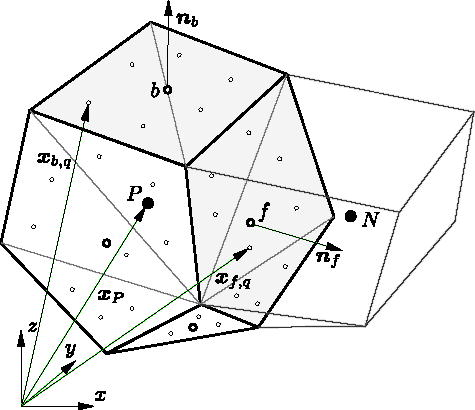
\includegraphics[scale=0.8]{figures/cv3D}  
    }
 	\caption{Representative convex polyhedral cell $P$ and neighbouring cell $N$}
 	\label{fig:cell}
\end{figure}
%
Accurate and robust flux integration is required over these arbitrary polyhedral volumes. 
To facilitate this, each polygonal face $f$ is subdivided into triangular subfaces, 
on which quadrature points $\bb{x}_{fg}$ are defined for numerical flux evaluation.
The fan triangulation method is adopted for face decomposition to minimise number of integration points.
Furthermore, each cell volume P is decomposed into tetrahedral
(in 3D) or triangular (in 2D) subelements, with volume quadrature points $\mathbf{x}_{\Omega,q}$ defined within each subelement.
A key advantage of this geometric framework is its unified treatment of arbitrary polyhedral topologies—all control 
volumes are handled consistently using the same reconstruction and integration procedures. 
%The discretization of the governing equations over a control volume P results in an algebraic stencil coupling 
%the centroid value $\mathbf{u}_P$ with the centroid values $\mathbf{u}_N$ of neighboring cells.

Before proceeding with the discretization of the volume and surface integrals, it is convenient to introduce the following sets of cell faces.
 The set of internal faces is denoted by $\mathcal{F}_P^{int}$, and the set of boundary faces by $\mathcal{F}_P^{bnd}$.
The boundary-face set $\mathcal{F}_P^{bnd}$ is further partitioned into three mutually disjoint subsets,
$\mathcal{F}_P^{bnd} := \mathcal{F}_P^{dip} \cup \mathcal{F}_P^{sym} \cup \mathcal{F}_P^{trac}$,
representing boundary faces where displacement ($\mathcal{F}_P^{dip}$), traction ($\mathcal{F}_P^{trac}$),
 or symmetry ($\mathcal{F}_P^{sym}$) conditions are prescribed.
%
%------------------------------------------------------------------------------
\subsection{Surface Integrals}
\label{sec:vol_int}
%------------------------------------------------------------------------------
%
% moram dodat kako se tezine racunaju
To ensure robustness, the method automatically switches to a cell-center decomposition when fan triangulation 
produces degenerate or near-zero-area triangles. 
For cell P, and its surfaces
\begin{equation}
\oint_{\Gamma_P} \bb{n} \cdot \bb{\sigma} \; \text{d}\Gamma_P 
= 
\sum_{f=1}^{f=N_f} \int_{\Gamma_f} \bb{n} \cdot \bb{\sigma} \; \text{d}\Gamma_f
\approx
\sum_{f=1}^{f=N_f} \bb{n}_{f} \cdot \left [ \sum_{q=1}^{q=N_q}\alpha_q \; \bb{\sigma}(\bb{x}_{f,q}) \right]\Gamma_f
\end{equation}
sigma ovisi o gradijentu, napisati preko konstoituivne relacije da se racuna sigma
\begin{equation}
\bb{\sigma}_s(\bb{x}_{f,q}) =   \mu (\nabla \bb{u})_{f,q} + \mu (\nabla \bb{u})^T_{f,q} +\lambda \text{tr}((\nabla \bb{u})_{f,q} )\mathbf{I}
\end{equation}
$(\nabla \bb{u})_{f,q}$ is given in section 3
%
%------------------------------------------------------------------------------
\subsection{Volume Integrals}
\label{sec:vol_int}
%------------------------------------------------------------------------------
%
Moram dodat kako se volumene tezine racuanaju da treba biti konzistentan
\begin{figure}[H]
 	\centering
    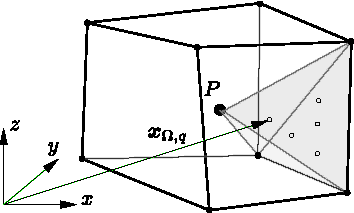
\includegraphics[scale=0.8]{figures/volumeTerm} 
 	\caption{Volume integration}
 	\label{fig:volumeTerm}
\end{figure}

%Volume mora biti konzistentan. Ciritari Nisikawu 2025.


%
%------------------------------------------------------------------------------
\subsection{Alpha Stabilisation}
\label{sec:vol_int}
%------------------------------------------------------------------------------
%
% In the latter section will be shown that discretisation withoud stabilisation is stable only on regular grids.
% The effect of stabilisaion can be obtained alternatuvely with large number of intehration poisnt and large stencil, howver alpha stabilisation
% introduced is more efficient and provide better stabilisation.
%Rhie-chow is second order- here we use Nishikawa alpha wich can be reduced to Rhie-chow stabilisation - see NK paper.
%UCNS3D: An open-source high-order finite-volume unstructured CFD, Nishiklawa 2025 paper
solver
\begin{equation}
\bb{t}_s = f_s \frac{2\mu +\lambda}{|\bb{d} \cdot \bb{n}|}(\bb{u}_{fN}^*-\bb{u}_{fP}^*)
\end{equation}

\begin{equation}
\bb{u}_{fP}^* = \bb{u}_P + \bb{d}_{Pf} \cdot (\nabla \bb{u})_P + \frac{1}{2}\bb{d}_{Pf}^2 \!:\! (\nabla \nabla \bb{u})_P + \frac{1}{6}\bb{d}_{Pf}^2 \!::\! (\nabla \nabla \nabla \bb{u})_P
\end{equation}
blabla
\begin{equation}
\bb{u}_{fN}^* = \bb{u}_N + \bb{d}_{Pf} \cdot (\nabla \bb{u})_N + \frac{1}{2}\bb{d}_{Nf}^2 \!:\! (\nabla \nabla \bb{u})_N + \frac{1}{6}\bb{d}_{Nf}^2 \!::\! (\nabla \nabla \nabla \bb{u})_N
\end{equation}
where $\bb{d}_{Pf}$ and $\bb{d}_{Nf}$  are defined as distance between face centre and cell centre, i.e. $\bb{d}_{fN}=(\bb{x}_f-\bb{x}_N)$ and is $\bb{d}_{fP}=(\bb{x}_f-\bb{x}_P)$ 



%
%------------------------------------------------------------------------------
\subsection{High order interpolation scheme}
\label{sec:ho_scheme}
%------------------------------------------------------------------------------
%

\subsection{Stencil}
slika lijevo (internal + boudnary molecule)
Slika desno cell centred molecule
Slka ispod za simetriju kako je implementirana


\subsection{Weight function}
\begin{equation}
w(\bb{x}, \bb{x}_N, k) = \frac{e^{-\tilde{d}^2k^2}-e^{-k^2}}{1-e^{-k^2}},
\end{equation}
where $\tilde{d}=\frac{d}{d_s}$
%
%------------------------------------------------------------------------------
\subsection{Boundary conditions}
\label{sec:bc}
%------------------------------------------------------------------------------
%


%
%%%%%%%%%%%%%%%%%%%%%%%%%%%%%%%%%%%%%%%%%%%%%%%%%%%%%%%%%%%%%%%%%%%%%%%%%%%%%%%
%      
\section{Solution Algorithm}
\label{sec:math_model}
%
%%%%%%%%%%%%%%%%%%%%%%%%%%%%%%%%%%%%%%%%%%%%%%%%%%%%%%%%%%%%%%%%%%%%%%%%%%%%%%%
%


%
%------------------------------------------------------------------------------
\subsection{Jacobian-free Newton-Krylov Algorithm}
\label{sec:vol_int}
%------------------------------------------------------------------------------
%


%
%%%%%%%%%%%%%%%%%%%%%%%%%%%%%%%%%%%%%%%%%%%%%%%%%%%%%%%%%%%%%%%%%%%%%%%%%%%%%%%
%        
\section{Test Cases}
\label{sec:test_cases}
%
%%%%%%%%%%%%%%%%%%%%%%%%%%%%%%%%%%%%%%%%%%%%%%%%%%%%%%%%%%%%%%%%%%%%%%%%%%%%%%%
%
% Test cases list (pros/cons having some case)
%
% MMS 
%     - 2D to show order of convergence in 2D. The behaviour is not the same as in 3D
%     - To show order of convergence
% Cantilever beam 
%     -to show that convergence is same with traction boundaries. Only 2D case. 
% Spherical cavity
%     - realistic 3D without source term which is overhead in mms
% Elliptic plate 
%     - to show parallel performance
% Cook's membarne
%    - Can be modelled with large (NeoHookean) and small deformations
%    - Can be used to show problems we have in 2D with hex mesh?
% Pressurised cylinder
%    - Can be modelled with large (Rivlin) and small deformations
% Idealised ventricle
%    - realstic 3D with large deformations
% Plate hole (maybe to replace with plateEllipticHole)
%The comparison of the performance of the reconstruction schemes discussed in
%319 the preceding section is done based on the convergence of the 𝐿- and 𝐿T norms of error
%320 in the reconstructed solution at flux integration points. This evaluation is carried out using
%321 model problems in 2-D with known exact solutions, and the specific exact solutions for
%322 the single-variable model problems examined are presented in Appendix B. The schemes
%323 are also tested using the supersonic vortex problem discussed earlier.

root mean square error
\begin{equation}
L_2 = \frac{1}{N_{\text{c}}}\sum_{i=1}^{N_{\text{c}}} |\Delta \phi_i|,
\end{equation}
and infinity norm representing the maximum absolute error
\begin{equation}
L_{\inf} = \max_{1 \leq i \leq N_{\text{c}}} |\Delta \phi_i|,
\end{equation}
where $\Delta \phi_i$ is the difference between expected and predicted solutions and $N_{\text{c}}$ is the overall number of computational points, i.e. cells.
Both norms are calculated for displacement magnitude $|\boldsymbol{u}|=\sqrt{u_x^2+u_y^2+u_z^2}$ and von Mises stress:
\begin{equation}
\sigma_{ekv}=\sqrt{\frac{1}{2}\left[  (\sigma_{xx}-\sigma_{yy})^2+(\sigma_{yy}-\sigma_{zz})^2+(\sigma_{zz}-\sigma_{xx})^2 \right]+3\left(\sigma_{xy}^2+\sigma_{yz}^2+\sigma_{zx}^2\right)}
\end{equation}
%
%------------------------------------------------------------------------------
\subsection{Case 1: Order Verification via the Manufactured Solution Procedure}
\label{case:mms}
%------------------------------------------------------------------------------
%
The first test case consists of a  $0.2 \times 0.2$ m square or $0.2 \times 0.2 \times 0.2$ m cube with linear elastic ($E = 200$ GPa, $\nu = 0.3$) properties.
A manufactured solution for displacement (Figure \ref{fig:mms_solution}) is employed in the form or polynomial, trigonometric \citep{Mazzanti2024} or mixed form \citep{Castrillo2022}:
\begin{itemize}
\item[•] \textbf{2D} 
\begin{eqnarray}
	\bb{u} =
	\begin{pmatrix}
 e^{x^2}\sin(y)\\
\ln(3+y)\cos(x)+\sin(y)\\
 0.
	\end{pmatrix}
\end{eqnarray}
\item[•] \textbf{3D - polynomial}

\begin{eqnarray}
	\bb{u} =
	\begin{pmatrix}
	a_x(x^3 + xy^2) \\
	a_y(y^3 + yz^2) \\
	a_z(z^3 + zx^2)
	\end{pmatrix}
\end{eqnarray}
where $a_x = 1\,\mu$m, $a_y = 1\,\mu$m, and $a_z = 1\,\mu$m.
\item[•] \textbf{3D - trigonometric}
 \begin{eqnarray}
	\bb{u} =
	\begin{pmatrix}
	a_x \sin(4\pi x) \sin(2\pi y) \sin(\pi z) \\
	a_y \sin(4 \pi x) \sin(2 \pi y) \sin(\pi z) \\
	a_z \sin(4 \pi x) \sin(2 \pi y) \sin(\pi z) 
	\end{pmatrix}
\end{eqnarray}
where $a_x = 2\,\mu$m, $a_y = 4\,\mu$m, and $a_z = 6\,\mu$m.
\end{itemize}
The Cartesian coordinates are given by $x$, $y$ and $z$.
The corresponding manufactured body force term ($\bb{f}_b$ in Equation \ref{eqn:momentum_lingeom}) can be found in authors previous publication \citep{Cardiff2025} or obtained by manufactured solution procedure.

\begin{figure}[H]
 	\centering
	\subfigure[Hexahedral mesh]
 	{
 		\label{fig:mms_solution}
    		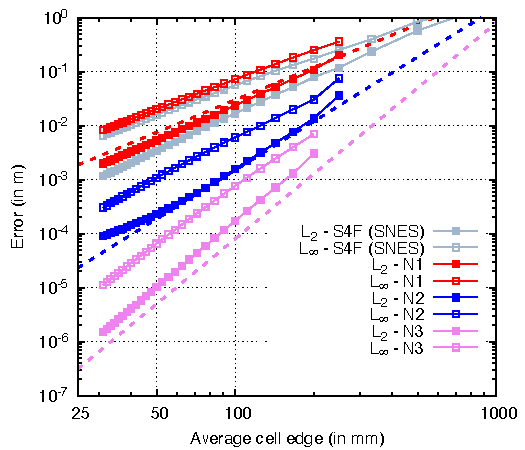
\includegraphics[scale=0.8]{figures/mms/2D/mms_dispErrors_ho-hex} 
    }
 	\subfigure[Tetrahedral structured mesh]
 	{
 		\label{fig:mms_mesh}
    		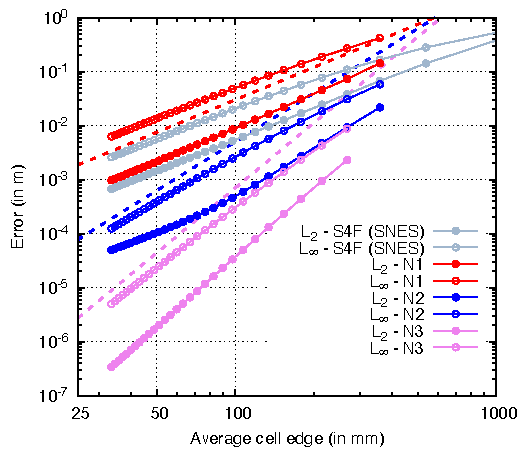
\includegraphics[scale=0.8]{figures/mms/2D/mms_dispErrors_ho-tet-struct}  
    }
    	\subfigure[Tetrahedral unstructured mesh]
 	{
 		\label{fig:mms_mesh}
    		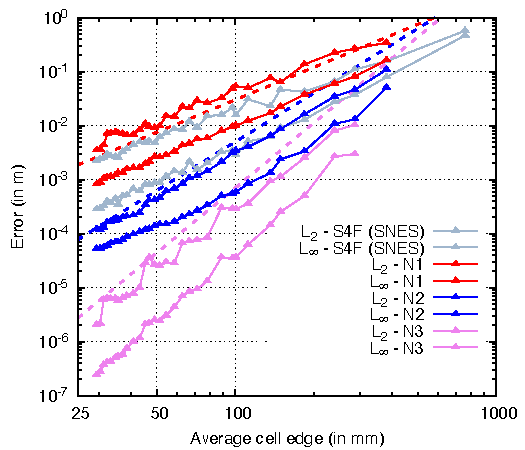
\includegraphics[scale=0.8]{figures/mms/2D/mms_dispErrors_ho-tet-unstruct}  
    }
 	\caption{Manufactured solution cube (2D case): error convergence for displacement magnitude}
 	\label{fig:xx}
 \end{figure}
 
 
\begin{figure}[H]
 	\centering
	\subfigure[Hexahedral mesh]
 	{
 		\label{fig:mms_solution}
    		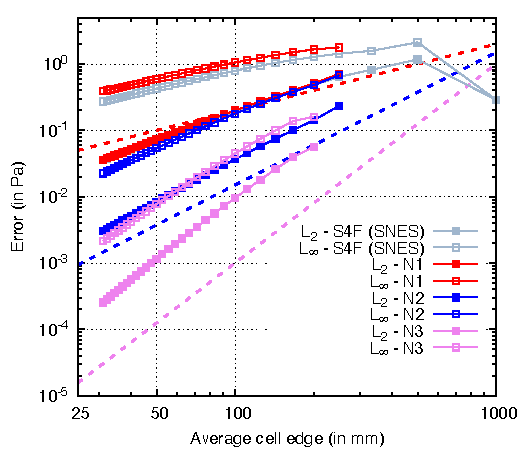
\includegraphics[scale=0.8]{figures/mms/2D/mms_stressErrors_ho-hex} 
    }
 	\subfigure[Tetrahedral structured mesh]
 	{
 		\label{fig:mms_mesh}
    		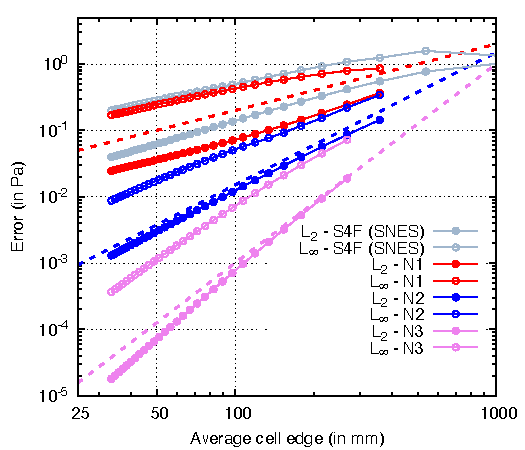
\includegraphics[scale=0.8]{figures/mms/2D/mms_stressErrors_ho-tet-struct}  
    }
    	\subfigure[Tetrahedral unstructured mesh]
 	{
 		\label{fig:mms_mesh}
    		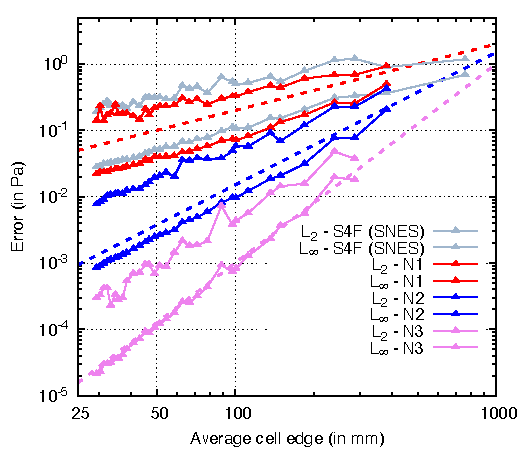
\includegraphics[scale=0.8]{figures/mms/2D/mms_stressErrors_ho-tet-unstruct}  
    }
 	\caption{Manufactured solution cube (2D case): error convergence for stress magnitude}
 	\label{fig:jj}
 \end{figure}
  

\begin{figure}[H]
 	\centering
	\subfigure[Hexahedral mesh]
 	{
 		\label{fig:mms_solution}
    		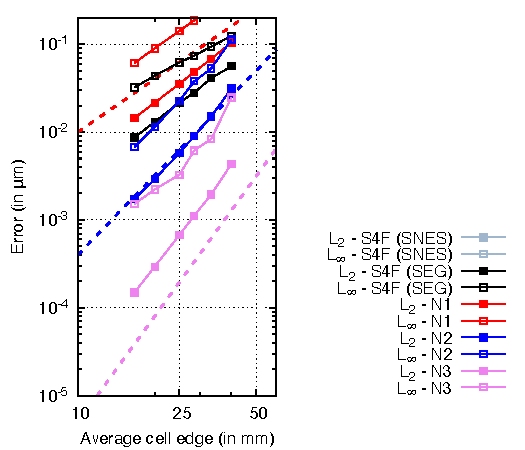
\includegraphics[scale=0.8]{figures/mms/3D/mms_dispErrors_ho-hex} 
    }
 	\subfigure[Tetrahedral structured mesh]
 	{
 		\label{fig:mms_mesh}
    		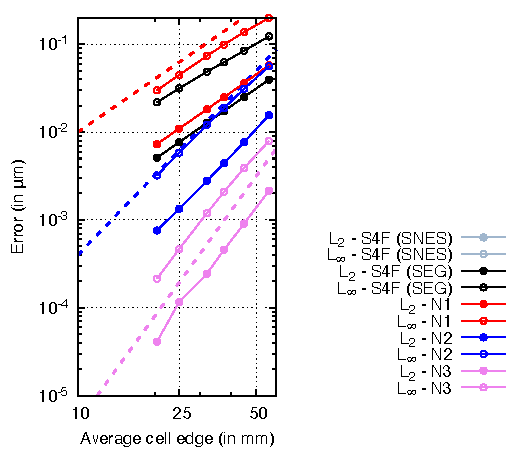
\includegraphics[scale=0.8]{figures/mms/3D/mms_dispErrors_ho-tet-struct}  
    }
     	\subfigure[Tetrahedral unstructured mesh]
 	{
 		\label{fig:mms_mesh}
    		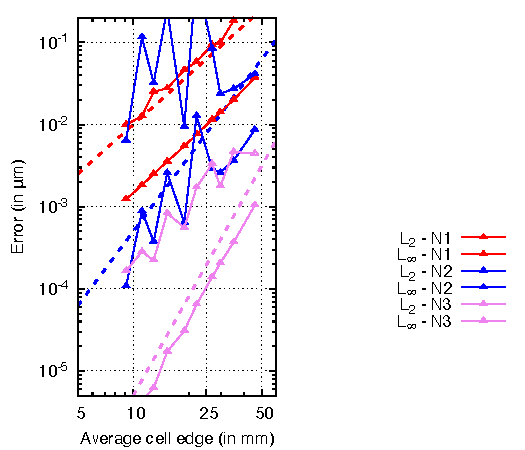
\includegraphics[scale=0.8]{figures/mms/3D/mms_dispErrors_ho-tet-unstruct}  
    }
    \subfigure[Polyhedral mesh]
 	{
 		\label{fig:mms_mesh}
    		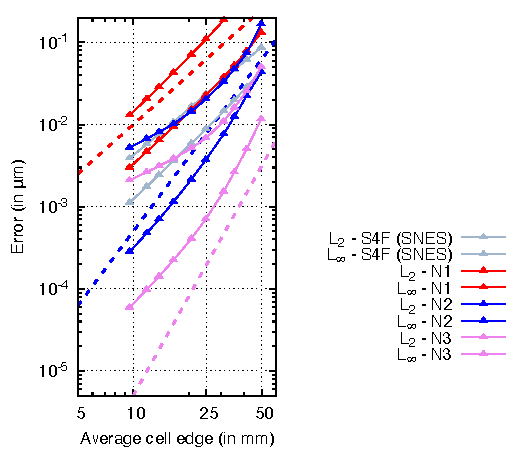
\includegraphics[scale=0.8]{figures/mms/3D/mms_dispErrors_ho-poly}  
    }
 	\caption{Manufactured solution cube (3D case): error convergence for displacement magnitude}
 	\label{fig:jj}
 \end{figure}
 
 
\begin{figure}[H]
 	\centering
	\subfigure[Hexahedral mesh]
 	{
 		\label{fig:mms_solution}
    		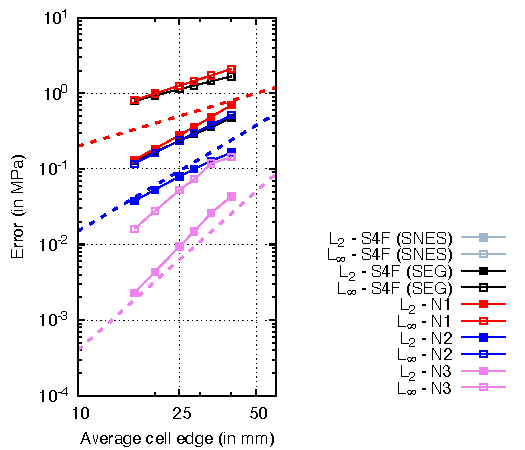
\includegraphics[scale=0.8]{figures/mms/3D/mms_stressErrors_ho-hex} 
    }
 	\subfigure[Tetrahedral structured mesh]
 	{
 		\label{fig:mms_mesh}
    		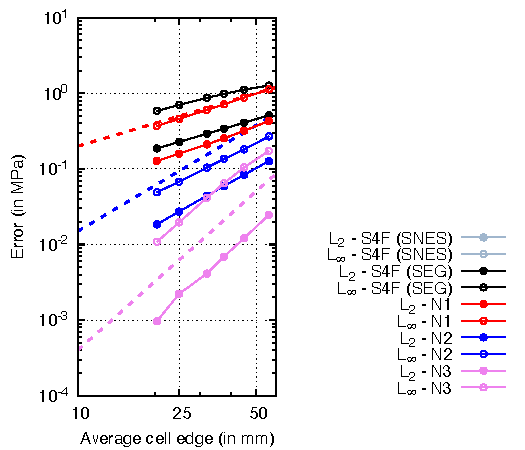
\includegraphics[scale=0.8]{figures/mms/3D/mms_stressErrors_ho-tet-struct}  
    }
    \subfigure[Polyhedral mesh]
 	{
 		\label{fig:mms_mesh}
    		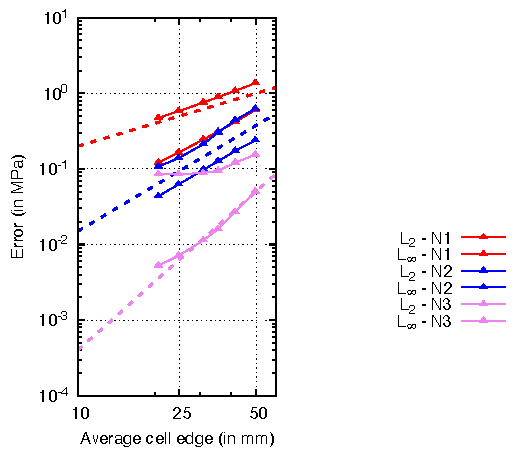
\includegraphics[scale=0.8]{figures/mms/3D/mms_stressErrors_ho-poly}  
    }
 	\caption{Manufactured solution cube (3D case): error convergence for stress magnitude}
 	\label{fig:jj}
 \end{figure}
%
%------------------------------------------------------------------------------
\subsection{Case 2: Cantilever beam}
%------------------------------------------------------------------------------
%
The test case geometry, shown in Fig. 6(a), is a rectangular beam with dimensions of $2$ m $\times$ $0.2$ m, a Young’s modulus of $E = 200$ GPa, and a Poisson’s ratio of $\nu = 0.3$. The top and bottom boundaries of the beam are traction-free, and plane strain conditions are assumed. The left end of the beam is constrained by the analytical displacement, while the right end is subjected to the corresponding analytical traction of (0, 1) MPa. This setup enables quantification of the difference between the predicted displacement and the analytical solution as a measure of convergence across the entire domain, rather than only at the beam end. Convergence is assessed using 15 successively refined grids.
%TO DO:
% - segregated solutions
% - Geometry and boundary conditions image
% - mesh images
%
\begin{figure}[H]
	\centering
	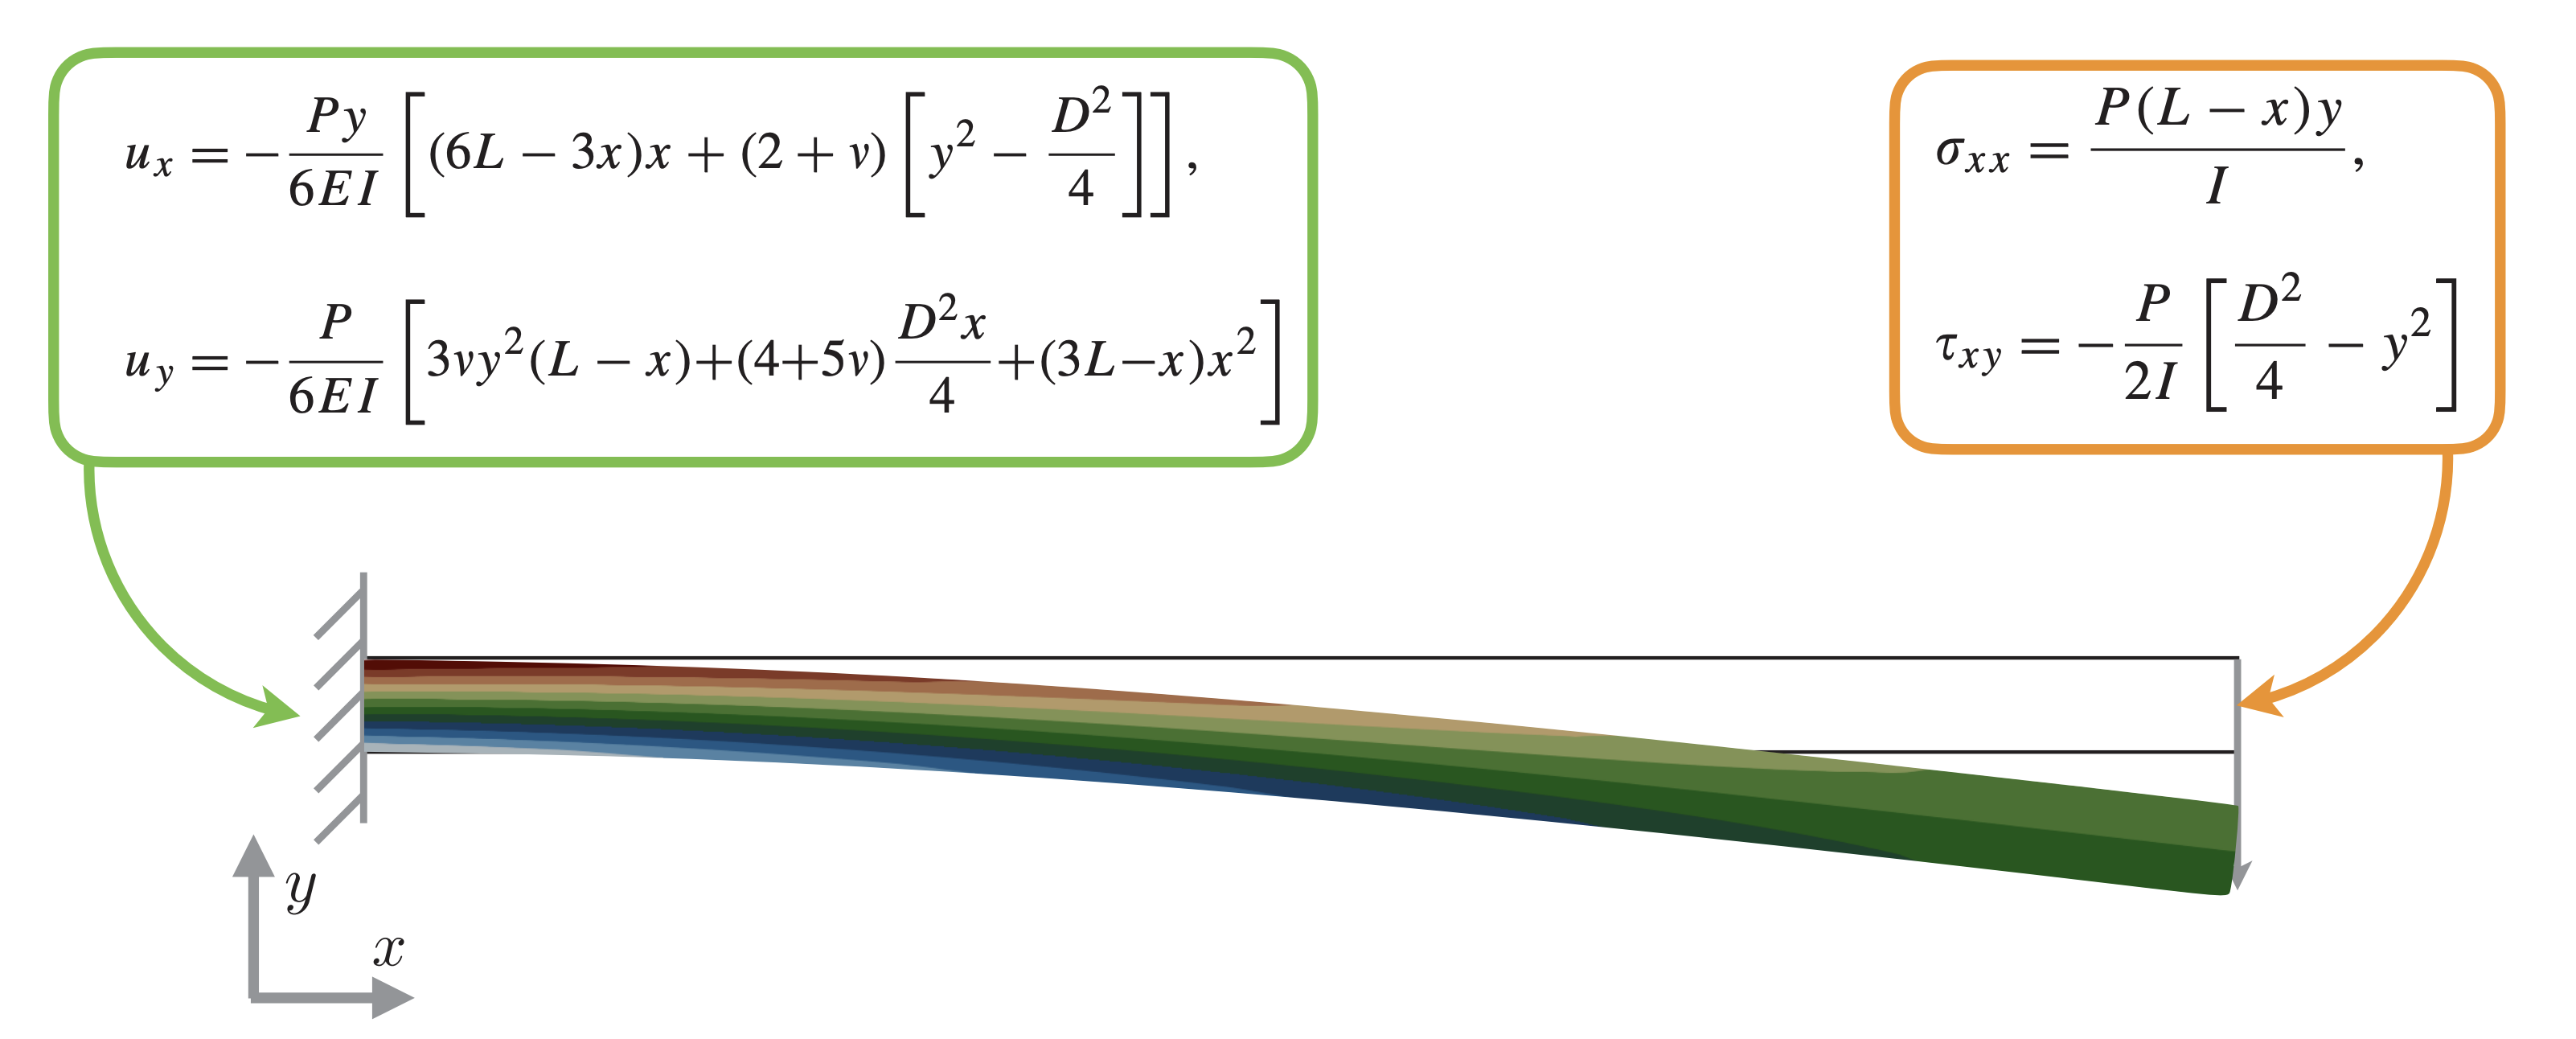
\includegraphics[width=0.7\textwidth]{figures/cantilever/cantilever.png} 
	\caption{Cantilever beam case: geometry and boundary conditions}
	\label{fig:cantilever}
\end{figure}

\begin{figure}[H]
 	\centering
	\subfigure[Hexahedral mesh]
 	{
 		\label{fig:mms_solution}
    		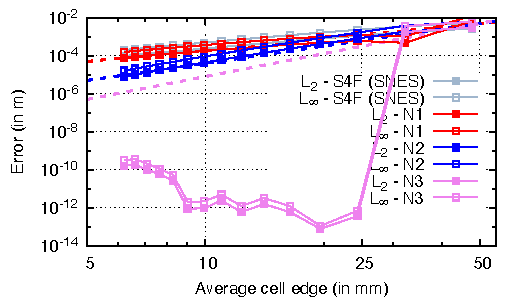
\includegraphics[scale=0.8]{figures/cantilever/dispErrors_hex} 
    }
 	\subfigure[Tetrahedral structured mesh]
 	{
 		\label{fig:mms_mesh}
    		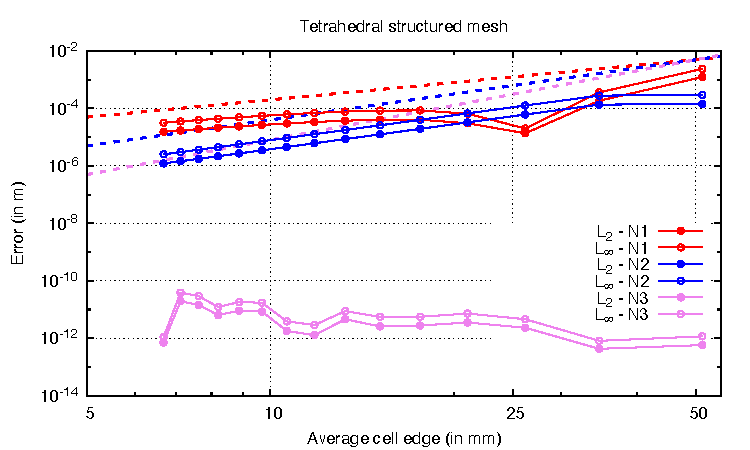
\includegraphics[scale=0.8]{figures/cantilever/dispErrors_tet-struct}  
    	}
    	\subfigure[Tetrahedral unstructured mesh]
 	{
 		\label{fig:mms_mesh}
    		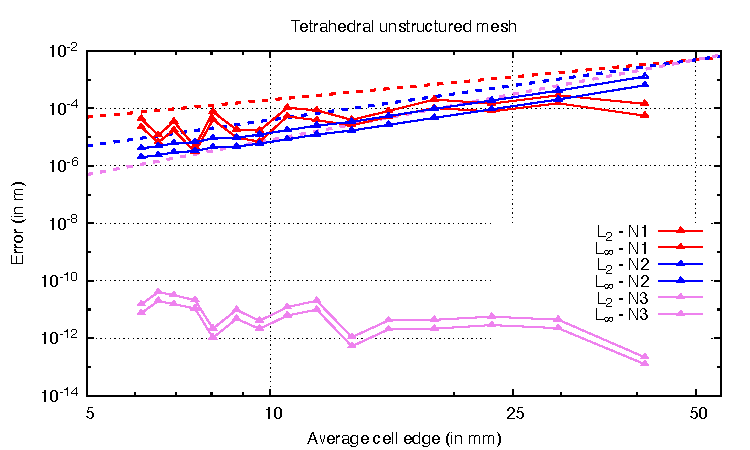
\includegraphics[scale=0.8]{figures/cantilever/dispErrors_tet-unstruct}  
    }
 	\caption{Cantilever beam case: displacement magnitude discretisation errors}
 	\label{fig:jj}
 \end{figure}

\begin{figure}[H]
 	\centering
	\subfigure[Hexahedral mesh]
 	{
 		\label{fig:mms_solution}
    		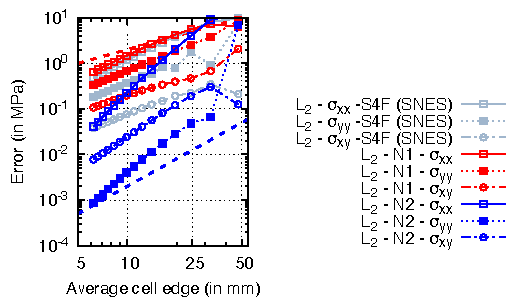
\includegraphics[scale=0.8]{figures/cantilever/stressErrors_hex} 
    }
 	\subfigure[Tetrahedral structured mesh]
 	{
 		\label{fig:mms_mesh}
    		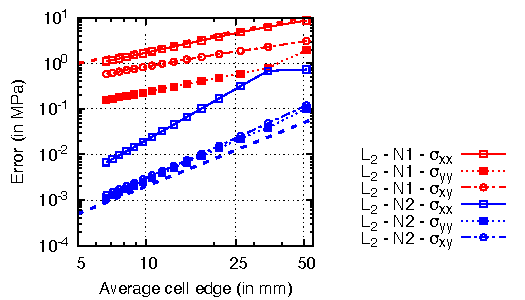
\includegraphics[scale=0.8]{figures/cantilever/stressErrors_tet-struct}  
    	}
    	\subfigure[Tetrahedral unstructured mesh]
 	{
 		\label{fig:mms_mesh}
    		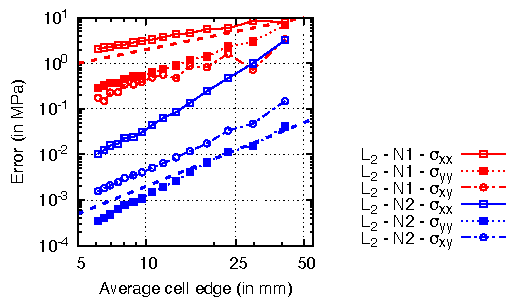
\includegraphics[scale=0.8]{figures/cantilever/stressErrors_tet-unstruct}  
    }
 	\caption{Cantilever beam case: $\sigma_{xx}$, $\sigma_{yy}$, $\sigma_{xy}$ stress discretisation errors. Results for $N=3$ are not shown because stress error is around $\sim$ $10^{-12}$}
 	\label{fig:uu}
 \end{figure}

\subsection{Case 3: Internally pressurised thick-walled cylinder}

In this case, a homogeneous thick-wall cylindrical pressure vessel with an inner radius $R_i = 7$ m, outer radius $R_o = 18.625$ m, and loaded internally with pressure $p = 100$ MPa is analysed. Two types of material are considered:
\begin{itemize}
\item[i.] Small strain, linear-elastic \cite{Bijelonja2006}: $E=10$ GPa, $\nu=0.3$.
\item[ii.] Finite strain, Mooney-Rivlin law \cite{Bijelonja2005a}: $c_{10} = 80$ MPa, $c_{01} = 20$ MPa, and $c_{11} = 0.0$ MPa and Poisson's ratio $\nu=0.49$
\end{itemize} 
The problem is considered plane stress, with the 2-D computational domain comprising a quarter of the cylinder geometry. The cylinder is discretised with series of unstructured tetrahedral grids. Gravitational and inertial effects are neglected. Linear elastic case is solved using one loading increment while hyperelastic case is solved using 100 equal loading increments. Analytical solutions are available in \cite{Timoshenko1970} and \cite{Green1992}.

%Pogledaj reference sve jesu li dobre, Green1992 je u bijelonji starija knjiha, vidi da li ima jos ovaj cejs.

\textcolor{red}{popraviiti slova na slici 8}


\begin{figure}[H]
 	\centering
 	\subfigure[Case geometry]
 	{
 		\label{fig:plateHole:a}
    		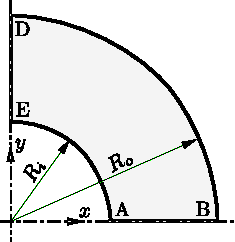
\includegraphics[scale=1]{figures/pressurisedCylinder-geometry} 
    }
	\subfigure[Tetrahedral mesh]
 	{
 		\label{fig:plateHole:b}
    		\includegraphics[scale=0.053]{figures/pressurisedCylinder-mesh} 
    }
 	\caption{Plate hole case geometry and mesh}
 	\label{fig:plateHole}
\end{figure}


\begin{figure}[H]
 	\centering
	\subfigure[Displacement convergence]
 	{
 		\label{fig:plateHole-disp:a}
    	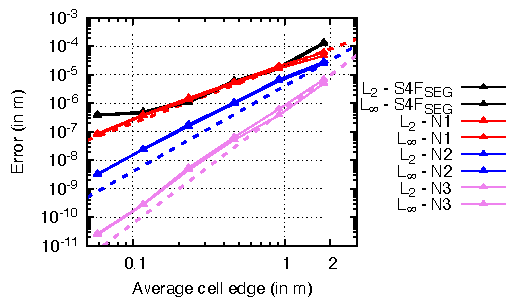
\includegraphics[scale=0.8]{figures/pressurisedCylinder-dispErrors_tet} 
    }
 	\subfigure[Stress convergence]
 	{
 		\label{fig:plateHole-disp:b}
    	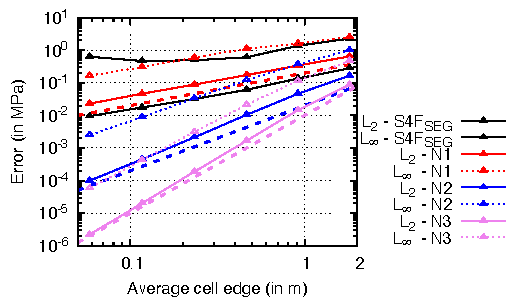
\includegraphics[scale=0.8]{figures/pressurisedCylinder-stressErrors_tet}  
    }
 	\caption{Pressurised cylinder case: displacement and stress magnitude discretisation errors for linear elastic material}
 	\label{fig:plateHole-disp}
 \end{figure}

\subsection{Case 4: Cooks membrane}

\subsection{Case 4: Plate hole}
% Case can be also found in:
% Finite volume method for stress analysis in complex domain
% Application of the nite volume method and unstructured meshes to linear elasticity
%
This benchmark problem consists of a thin, infinitely large plate with a circular hole, subjected to uniaxial tension. Owing to the symmetry of the geometry and loading, only one quarter of the plate is modeled as a finite domain. To minimize the influence of the finite computational boundaries, the exact tractions obtained from the analytical solution \cite{Demirdzic1997} are prescribed on the outer edges BC and CD. Symmetry boundary conditions are applied on boundaries AB and DE, while zero traction is specified on the hole boundary. The material properties are defined by a Young’s modulus of $E = 200 \,\text{GPa}$ and a Poisson’s ratio of $\nu = 0.3$.
%
\begin{figure}[H]
 	\centering
 	\subfigure[Case geometry]
 	{
 		\label{fig:plateHole:a}
    		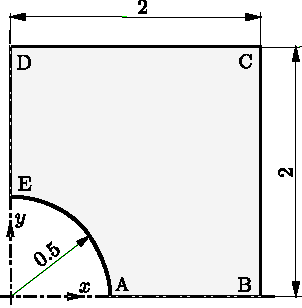
\includegraphics[scale=1]{figures/plateHole-geometry} 
    }
	\subfigure[Hexahedral mesh]
 	{
 		\label{fig:plateHole:b}
    		\includegraphics[scale=0.06]{figures/plateHole-hexmesh} 
    }
 	\subfigure[Tetrahedral mesh]
 	{
 		\label{fig:plateHole:a}
    	\includegraphics[scale=0.06]{figures/plateHole-tetmesh}  
    }
 	\caption{Plate hole case geometry and mesh}
 	\label{fig:plateHole}
\end{figure}
%
Hexahedral mesh with N3 needs 20 neighbours to avoid ill conditioning. This results in lower slope for displacement but not affecting the stresses. I'm not sure why S4F results flatten on finer meshes.
%
\begin{figure}[H]
 	\centering
	\subfigure[Hexahedral mesh]
 	{
 		\label{fig:plateHole-disp:a}
    	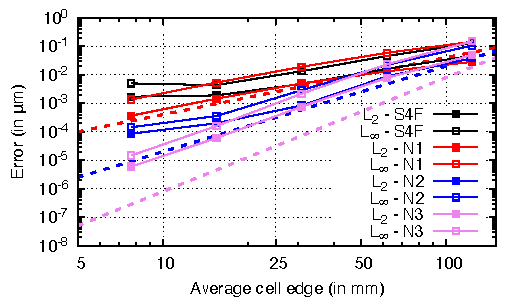
\includegraphics[scale=0.8]{figures/plateHole-dispErrors_hex} 
    }
 	\subfigure[Tetrahedral mesh]
 	{
 		\label{fig:plateHole-disp:b}
    	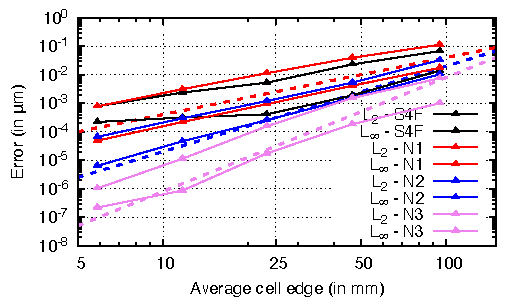
\includegraphics[scale=0.8]{figures/plateHole-dispErrors_tet-unstruct}  
    }
 	\caption{Plate hole case: displacement magnitude discretisation errors}
 	\label{fig:plateHole-disp}
 \end{figure}
 
\begin{figure}[H]
 	\centering
	\subfigure[Hexahedral mesh]
 	{
 		\label{fig:plateHole-stress:a}
    	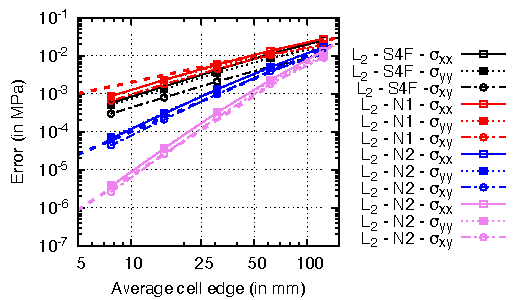
\includegraphics[scale=0.8]{figures/plateHole-stressErrors_hex} 
    }
 	\subfigure[Tetrahedral mesh]
 	{
 		\label{fig:plateHole-stress:a}
    	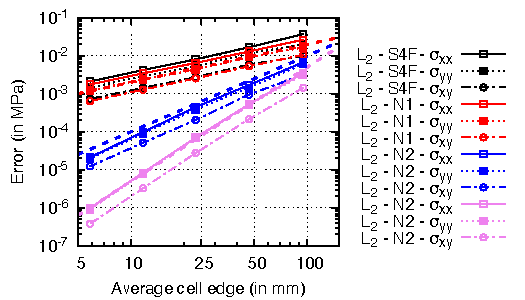
\includegraphics[scale=0.8]{figures/plateHole-stressErrors_tet-unstruct}  
   	}
 	\caption{Plate hole case: $\sigma_{xx}$, $\sigma_{yy}$, $\sigma_{xy}$ stress discretisation errors.}
 	\label{fig:plateHole-stress}
 \end{figure}
 
 
 
\subsection{Case 5: Elliptic plate}
\subsection{Case 6: Spherical cavity}
\subsection{Case 7: Idealised ventricle}

\subsection{Error-cost relationship}

\subsection{Stabilisation scheme}

\subsection{Effects of poor interpolation conditioning}

Plate hole sa hex mrezom tu staviti i objasniti sto se desava u 2D-u sa kondicijskim brojem interpolacije

\subsection{Code parallelisation}
%- analytical solution on boundaries
%Case 3: Elliptic plate (kako izvuc rezultate?)


%
%Math model and numerical methods
%- General governing equation -> unknown D; limit ourselves to compressibility

%% \subsection{Governing Equations} \label{sec:governing_eqn}

%% In this work, interest is restricted to Lagrangian formulations of the conservation of linear momentum.
%% Assuming small strains, the linear geometry formulation is expressed in strong integral form as:
%% \begin{eqnarray} \label{eqn:momentum_lingeom}
%%     \int_{\Omega} \rho \frac{\partial^2 \bb{u} }{\partial t^2} \, d\Omega
%%     =
%%     \oint_{\Gamma} \bb{n} \cdot \bb{\sigma}_s \,  d\Gamma
%%     + \int_{\Omega}  \bb{f}_b \, d\Omega
%% \end{eqnarray}
%% where $\Omega$ is the volume of an arbitrary body bounded by a surface $\Gamma$ with outwards pointing normal $\bb{n}$.
%% The density is $\rho$, $\bb{u}$ is the displacement vector, $\bb{\sigma}_s$ is the engineering (small strain) stress tensor, and $\bb{f}_b$ is a body force per unit volume, e.g., $\rho \bb{g}$, where $\bb{g}$ is gravity.

%% More generally,  linear momentum conservation can be expressed in a nonlinear geometry form, which is suitable for finite strains.
%% Two equivalent nonlinear geometry forms are common: the \emph{total} Lagrangian form:
%% \begin{eqnarray} \label{eqn:momentum_TL}
%%     \int_{\Omega_o} \rho_o \frac{\partial^2 \bb{u} }{\partial t^2} d\Omega_o
%%     =
%%     \oint_{\Gamma_o} \left( J \bb{F}^{-\text{T}} \cdot \bb{n}_o \right) \cdot \bb{\sigma} \ d\Gamma_o
%%     + \int_{\Omega_o}  \bb{f}_b \, d\Omega_o
%% \end{eqnarray}
%% and the \emph{updated} Lagrangian form:
%% \begin{eqnarray} \label{eqn:momentum_UL}
%%     \int_{\Omega_u} \frac{\partial }{\partial t} \left( \rho_u \frac{\partial \bb{u} }{\partial t} \right) d\Omega_u
%%     = \oint_{\Gamma_u}(j\bb{f}^{-\text{T}}\cdot{\bb{n}_u)\cdot \bb{\sigma}}\ d\Gamma_u
%%     + \int_{\Omega_u}  \bb{f}_b \, d\Omega_u
%% \end{eqnarray}
%% where subscript $o$ indicates quantities in the initial reference configuration, and subscript $u$ indicates quantities in the updated configuration.
%% The true (Cauchy) stress tensor is indicated by $\bb{\sigma}$.
%% The deformation gradient is defined as $\bb{F} = \textbf{I} + (\bb{\nabla} \bb{u})^{\text{T}}$ and its determinant as $J = \text{det}(\bb{F})$.
%% Similarly, the \emph{relative} deformation gradient is given in terms of the displacement \emph{increment} as $\bb{f}=\textbf{I} + \left[\bb{\nabla}(\Delta \bb{u}) \right]^{\text{T}}$ and its determinant as $j = \text{det}(\bb{f})$.
%% The displacement increment is the change in displacement between the current time step and the previous time step when the time interval is discretised into a finite number of steps.

%% %The two forms are connected through Nanson’s formula \cite{bathe_finite_1996}, which relate the deformed area vector $\bb{\Gamma}$ with the initial area vector $\bb{\Gamma}_{o}$:
%% %\begin{equation}
%% %    \bb{\Gamma} = J\bb{F}^{-\text{T}}\cdot\bb{\Gamma}_o
%% %\end{equation}
%% %Although the total Lagrangian approach is a viable option for wire drawing, the current work adopts the updated Lagrangian approach as developing Eulerian-type upstream and downstream conditions (Section \ref{sec:euler_BCs}) is conceptually easier in an updated Lagrangian formulation.


%% The governing equations are complemented by boundary conditions, with three types considered here: prescribed displacement, prescribed traction, and symmetry.
%% The definition of the engineering stress ($\bb{\sigma}_s$) and true stress ($\bb{\sigma}$) in Equations \ref{eqn:momentum_lingeom}, \ref{eqn:momentum_TL} and \ref{eqn:momentum_UL} is given by a chosen mechanical law.
%% Five mechanical laws are considered in this work, as briefly outlined in Appendix \ref{app:mechLaws}: linear elasticity (Hooke's law), three forms of hyperelasticity (St.\,Venant-Kirchhoff, neo-Hookean, and Guccione), and neo-Hookean $J_2$ hyperelastoplasticity.


%% %%--------------------------------------------------------------------------------------------------------------------%%
%% \subsection{Newton-Type Solution Methods}
%% %%--------------------------------------------------------------------------------------------------------------------%%
%% To facilitate the comparison between the classic segregated solution algorithm and the proposed Jacobian-free Newton-Krylov algorithm, the governing linear momentum conservation (Equations \ref{eqn:momentum_lingeom}, \ref{eqn:momentum_TL} and \ref{eqn:momentum_UL}) is expressed in the general form:
%% \begin{eqnarray} \label{eqn:residual}
%% 	    \bb{R}(\bb{u}) = \bb{0}
%% \end{eqnarray}
%% where $\bb{R}$ represents the \emph{residual} (imbalance) of the equation, which is a function of the primary unknown field.
%% For example, in the linear geometry case, the residual is given as
%% \begin{eqnarray}
%%     \bb{R}(\bb{u})
%%     \;=\;
%%     \oint_{\Gamma} \bb{n} \cdot \bb{\sigma}_s(\bb{u}) \,  d\Gamma
%%     + \int_{\Omega}  \rho \bb{g} \, d\Omega
%%     -  \int_{\Omega} \rho \frac{\partial^2 \bb{u} }{\partial t^2} \, d\Omega
%%     \;=\; \bb{0}
%% \end{eqnarray}
%% where the dependence of the stress tensor on the solution vector is made explicitly clear: $\bb{\sigma}_s(\bb{u})$.



%% In Newton-type methods, a Taylor expansion about a current point $\bb{u}_k$ can be used to solve Equation \ref{eqn:residual} \cite{Knoll2004}:
%% \begin{eqnarray}
%% 	\bb{R}(\bb{u}_{k+1}) = \bb{R}(\bb{u}_{k}) \;+\;  \bb{R}'(\bb{u}_{k}) (\bb{u}_{k+1} - \bb{u}_{k}) \;+\; \text{H.O.T.} = \bb{0}
%% \end{eqnarray}
%% Neglecting the higher-order terms ($\text{H.O.T.}$) yields the strict Newton method in terms of an iteration over a sequence of linear systems: 
%% \begin{eqnarray} \label{eq:NewtonRaphson}
%% 	\bb{J}(\bb{u}_k) \delta \bb{u} &=& -\bb{R}(\bb{u}_k), \notag \\
%% 	\bb{u}_{k+1} &=& \bb{u}_k + s \, \delta \bb{u}, \notag \\
%% 	\quad
%% 	k &=& 0,1,...
%% %    \label{eq:NewtonRaphsonA}
%% %    \overbrace{\left[ \frac{\partial \mathcal{R}(\bb{u})}{\partial \bb{u}} \right]_n}^{\mathcal{J}} \Delta \bb{u} = -\mathcal{R}(\bb{u})_n \\
%% %    \label{eq:NewtonRaphsonB}
%% %    \bb{u}_{n+1} = \bb{u}_{n} + \alpha \Delta \bb{u}
%% \end{eqnarray}
%% where $\bb{J} \equiv \bb{R}' \equiv \partial \bb{R}/\partial \bb{u}$ is the Jacobian matrix.
%% Starting the Newton procedure requires the specification of $\bb{u}_0$.
%% %is iteratively solved by linearisation about the current value of the solution, leading to a linear system and iterative update of the solution vector:
%% %\begin{eqnarray}
%% %    \label{eq:NewtonRaphsonA}
%% %    \overbrace{\left[ \frac{\partial \mathcal{R}(\bb{u})}{\partial \bb{u}} \right]_n}^{\mathcal{J}} \Delta \bb{u} = -\mathcal{R}(\bb{u})_n \\
%% %    \label{eq:NewtonRaphsonB}
%% %    \bb{u}_{n+1} = \bb{u}_{n} + \alpha \Delta \bb{u}
%% %\end{eqnarray}
%% %where subscript $n$ indicates the outer (Newton) iteration index.
%% The scalar $s > 0$ can be chosen to improve convergence, for example, using a line search or under-relaxation/damping procedure, and is equal to unity in the classic Newton-Raphson approach.
%% Iterations are performed over this system until the residual $\bb{R}(\bb{u}_k)$ and solution correction $\delta \bb{u}$ are sufficiently small, with appropriate normalisation.

%% %\hl{$\Delta u$: we are using in two ways: increment and correction. Fix this!}
%% %\hl{KnollKeyes give a nice concise description of Newton: check}

%% For problems with $N$ scalar equations and $N$ scalar unknowns, the residual $\bb{R}$ and solution $\bb{u}$ vectors have dimensions of $N \times 1$. %, while the Jacobian matrix has dimensions of $N \times N$.
%% %In contrast, for vector problems, like the solid mechanics problems considered in this work, the residual and solution vectors have dimensions of $N_d N \times 1$ and the Jacobian matrix has dimensions of $N_d N \times N_d N$, where $N_d$ is the geometric dimension of the problem, e.g. $N_d = 2$ for 2-D and $N_d = 3$ for 3-D.
%% The components of the $N \times N$ Jacobian are
%% \begin{eqnarray} \label{eq:J}
%% 	{J}_{ij} = \frac{\partial {R}_i (\bb{u})}{\partial u_j}
%% \end{eqnarray}

%% The current work focuses on vector problems, where the governing momentum equation is formulated in terms of the unknown displacement solution vector.
%% In this case, Equation \ref{eq:J} refers to the individual scalar components of the residual, solution, and Jacobian.
%% That is, for 3-D analyses, the residual takes the form
%% \begin{eqnarray}
%% 	\bb{R}(\bb{u}) = \left\{ R_1^x, R_1^y, R_1^z, R_2^x, R_2^y, R_2^z, ..., R_n^z \right\}
%% \end{eqnarray}
%% and the solution takes the form
%% \begin{eqnarray}
%% 	\bb{u} = \left\{ u_1^x, u_1^y, u_1^z, u_2^x, u_2^y, u_2^z, ..., u_n^z \right\}
%% \end{eqnarray}
%% In practice, it is often more practical and efficient to form and store the residual, solution and Jacobian in a \emph{blocked} manner, where the residual and solution can be considered as vectors of vectors.
%% Similarly, the Jacobian can be formed in terms of sub-matrix block coefficients.

%% In the strict Newton procedure, the residuals converge at a quadratic rate when the current solution is close to the true solution; that is, the iteration error decreases proportionally to the square of the error at the previous iteration.
%% Once the method gets sufficiently close to the true solution, the number of correct digits in the approximation roughly doubles with each iteration. 
%% However, quadratic convergence is only possible when using the exact Jacobian.
%% In contrast, a quasi-Newton method uses an approximation to the Jacobian, sacrificing strict quadratic convergence in an attempt to produce an overall more computationally efficient procedure.
%% From this perspective, the segregated solution algorithm commonly employed in finite volume solid mechanics can be viewed as a quasi-Newton method, where an approximate Jacobian replaces the exact Jacobian: 
%% \begin{eqnarray} \label{eq:Seg}
%%     \bb{\tilde{J}}(\bb{u}_k) \;\delta \bb{u} = -\bb{R}(\bb{u}_k)
%% \end{eqnarray}
%% In this case, the approximate Jacobian $\bb{\tilde{J}}$ comes from the compact stencil discretisation of a simple diffusion (Laplacian) term inertia terms.
%% A benefit of this approach is that the inter-component coupling is removed from the Jacobian, allowing the solution of three smaller scalar systems rather than one larger vector system in 3-D (or two smaller systems in 2-D).

%% A fully explicit procedure can also be viewed from this perspective by selecting a \emph{diagonal} approximate Jacobian $\bb{\tilde{D}}$ (only the inertia term), making the solution of the linear system trivial:
%% \begin{eqnarray} \label{eq:exp}
%%     \bb{\tilde{D}}(\bb{u}_k) \;\delta \bb{u} = -\bb{R}(\bb{u}_k)
%% \end{eqnarray}


%% %%--------------------------------------------------------------------------------------------------------------------%%
%% \subsection{Cell-Centred Finite Volume Discretisation}
%% \label{sec:discretisation}
%% %%--------------------------------------------------------------------------------------------------------------------%%
%% In this work, a nominally second-order cell-centred finite volume discretisation is employed.
%% % based on previously described work, for example, \citep{Cardiff2017, Batistic2022, Tukovic2013, Jasak2000}.
%% %Consequently, only a summary of the discretisation is presented below.
%% The solution domain is discretised in both space and time.
%% The total simulation period is divided into a finite number of time increments, denoted as $\Delta t$, and the discretised governing momentum equation is solved iteratively in a time-marching fashion.
%% %The spatial domain is partitioned into a finite number of contiguous convex polyhedral cells.
%% The spatial domain is partitioned into a finite set $\mathcal{P}$ of contiguous convex polyhedral cells, where each cell is denoted by $P \in \mathcal{P}$.
%% The number of cells in the mesh is indicated by $|\mathcal{P}|$.
%% A representative cell $P$ is shown in Figure~\ref{fig:cell}.
%% The set of all faces of cell $P$ is denoted by $\mathcal{F}_P$. This set is further subdivided into two disjoint subsets:
%% \begin{itemize}
%%     \item \textbf{Internal Faces} ($\mathcal{F}^{\text{int}}_P$): Faces that are shared with neighbouring cells.
%%     \item \textbf{Boundary Faces} ($\mathcal{F}^{\text{bnd}}_P$): Faces that lie on the boundary of the spatial domain.
%%     The boundary faces of cell $P$ are further classed into three disjoint sets, $\mathcal{F}^{\text{bnd}}_P \coloneqq \mathcal{F}^{\text{disp}}_P \cup \mathcal{F}^{\text{trac}}_P \cup \mathcal{F}^{\text{symm}}_P$, representing boundary faces where displacement ($\mathcal{F}^{\text{disp}}_P$), traction ($\mathcal{F}^{\text{trac}}_P$) and symmetry ($\mathcal{F}^{\text{symm}}_P$) conditions are prescribed.
%%        % \quad \text{with} \quad \mathcal{F}^{\text{disp}}_P \cap \mathcal{F}^{\text{trac}}_P = \mathcal{F}^{\text{disp}}_P \cap \mathcal{F}^{\text{symm}}_P = \mathcal{F}^{\text{trac}}_P \cap \mathcal{F}^{\text{symm}}_P = \emptyset.$
%% \end{itemize}
%% Each internal face $f_i \in \mathcal{F}^{\text{int}}_P$ corresponds to a neighbouring cell $N_{f_i} \in \mathcal{N}_P$, where $\mathcal{N}_P$ is the set of all neighbouring cells of $P$. The outward unit normal vector associated with an internal face $f_i$ is denoted by $\mathbf{n}_{f_i}$, while the outward unit normal vector associated with a boundary face $b_i$ is denoted by $\mathbf{n}_{b_i}$.
%% The vector $\mathbf{d}_{f_i}$ connects the centroid of cell $P$ with the centroid of the neighbouring cell $N_{f_i}$, whereas the vector $\mathbf{d}_{b_i}$ connects the centroid of cell $P$ with the centroid of boundary face ${b_i}$.
%% For convenience, we will also define the set of all faces of cell $P$ excluding those on a traction boundary as $\mathcal{F}_P^{\text{non-trac}} \coloneqq \mathcal{F}_P^{\text{int}} \cup \mathcal{F}_P^{\text{disp}} \cup \mathcal{F}_P^{\text{symm}}$.
%% %The proposed solution discretisation follows closely the approach of \citet{cardiff_lagrangian_2017}; consequently, only an overview of the final discretised form of equations and adopted solution algorithm are given below.
%% \begin{figure}[htbp]
%% 	\centering
%% %	\subfigure[Magnitude of the manufactured displacement solution]
%% %	{
%% %		\label{fig:mms_solution}
%%    		\includegraphics[width=\textwidth]{figures/cell} 
%% %   	}
%% %	\subfigure[Polyhedral mesh with $1\,000$ cells]
%% %	{
%% %		\label{fig:mms_mesh}
%% %   		\includegraphics[height=0.45\textwidth]{figures/mms_mesh}  
%% %   	}
%% 	\caption{Representative convex polyhedral cell $P$ and neighbouring cell $N_{f_i}$, which share a face $f_i$.}
%% 	\label{fig:cell}
%% \end{figure}


%% %The conservation equation (Equations \ref{eqn:momentum_lingeom}, \ref{eqn:momentum_TL}, or \ref{eqn:momentum_UL}) is applied to each cell $\mathcal{P}$ and discretised in terms of the displacement at the centroid of the cell $\bb{u}_P$ and the displacements at the centroids of the neighbouring cells $\bb{u}_{N_{f_i}} \in N_i$.
%% The conservation equation (Equations \ref{eqn:momentum_lingeom}, \ref{eqn:momentum_TL}, or \ref{eqn:momentum_UL}) is applied to each cell $P$ and discretised in terms of the displacement at the centroid of the cell $\boldsymbol{u}_P$ and the displacements $\boldsymbol{u}_{N_{f_i}}$ at the centroids of the neighbouring cells.
%% % $\boldsymbol{u}_{N_{f_i}} \in \mathcal{U}_{\mathcal{N}_P}$, where $\mathcal{U}_{\mathcal{N}_P}$ represents the set of such displacements.
%% Proceeding with the discretisation, the volume and surface integrals in the governing equation are approximated by algebraic equations as described below.


%% \subsubsection{Volume Integrals}
%% To discretise the volume integrals, the integrand $\bb{\phi}$ is assumed to locally vary according to a truncated Taylor series expansion about the centroid of cell $P$:
%% \begin{eqnarray}
%% 	\bb{\phi}(\bb{x})  \approx \bb{\phi}_P + (\bb{x} - \bb{x}_P) \cdot \nabla \bb{\phi}_P
%% \end{eqnarray}
%% where subscript $P$ indicates a value at the centroid of the cell $P$.
%% %assuming a linear variation of the integrand across the cell, the mid-point rule approximates the integral in terms of the cell centre value.
%% Consequently, volume integrals over a cell $P$ can be approximated to second-order accuracy as
%% \begin{eqnarray} \label{eq:volume_integral}
%% 	\int_{\Omega_P} \bb{\phi} \, d \Omega_P
%% 		&\approx& \int_{\Omega_P}  \left[ \bb{\phi}_P + (\bb{x} - \bb{x}_P) \cdot \nabla \bb{\phi}_P \right] d \Omega_P \notag \\
%% %		&\approx& \int_{\mathrm{\Omega}}  \bb{\phi}_P d\mathrm{\Omega}  + \int_{\mathrm{\Omega}}  (\bb{x} - \bb{x}_P) \cdot \nabla \bb{\phi}_P d\mathrm{\Omega} \notag \\
%% 		&\approx& \bb{\phi}_P \Omega_P
%% \end{eqnarray}
%% where $\Omega_P$ is the volume of cell $P$ and $\int_{\Omega_P} (\bb{x} - \bb{x}_P) d\Omega_P \equiv 0$ by definition of the cell centroid.
%% This approximation corresponds to the midpoint rule and one point quadrature.

%% Using Equation \ref{eq:volume_integral}, the inertia term (e.g. left-hand side term of Equation \ref{eqn:momentum_lingeom}) becomes
%% \begin{eqnarray} \label{eq:inertia}
%% 	\int_{\Omega_P} \rho \frac{\partial \bb{u} }{\partial t}  d \Omega_P
%% %	\;&\approx&\;
%% %	\int_{\mathrm{\Omega}} \rho \left[ \frac{\partial \bb{u} }{\partial t}_P + (\bb{x} - \bb{x}_P) \cdot \nabla \frac{\partial \bb{u} }{\partial t}_P \right] d\mathrm{\Omega} \notag \\
%% 	\;&\approx&\;
%% 	\rho_P \left(\frac{\partial^2 \bb{u} }{\partial t^2}\right)_P  \Omega_P
%% \end{eqnarray}
%% Similarly, the body force term (e.g. the second term on the right-hand side of Equation \ref{eqn:momentum_lingeom}) becomes:
%% \begin{eqnarray}
%% 	\int_{\Omega_P} \, \rho \, \bb{g} \,  d \Omega_P
%% 	\;&\approx&\;
%% 	\rho_P \, \bb{g}\,  \Omega_P
%% \end{eqnarray}
%% %where subscript $P$ indicates a quantity at the cell centre.
%% The discretisation of the acceleration in Equation \ref{eq:inertia} can be achieved using one of many finite difference schemes, e.g. first-order Euler, second-order backwards, or second-order Newmark-beta.
%% In the current work, the second-order backwards (BDF2) scheme is used:
%% %\begin{eqnarray}
%% %	 \left(\frac{\partial^2 \bb{u} }{\partial t^2}\right)_P
%% %	 &\approx& \frac{3\bb{v}_{t+1} - 4\bb{v}_{t} + \bb{v}_{t-1}}{2\Delta t} \notag \\
%% %	&\approx& \frac{3\left( \frac{3\bb{u}_{t+1} - 4\bb{u}_{t} + \bb{u}_{t-1}}{2\Delta t} \right) - 4\bb{v}_{t} + \bb{v}_{t-1}}{2\Delta t}
%% %\end{eqnarray}
%% \begin{eqnarray} \label{eq:inertia2}
%% 	\left(\frac{\partial^2 \boldsymbol{u}_P}{\partial t^2}\right)_P
%% 	&\approx& \frac{3\boldsymbol{v}_P^{[t+1]} - 4\boldsymbol{v}_P^{[t]} + \boldsymbol{v}_P^{[t-1]}}{2\Delta t} \notag \\
%% 	&\approx&
%% 	\frac{3\left( 
%% 		\dfrac{3\boldsymbol{u}_P^{[t+1]} - 4\boldsymbol{u}_P^{[t]} + \boldsymbol{u}_P^{[t-1]}}{2\Delta t} 
%% 		\right) 
%% 	- 4\boldsymbol{v}_P^{[t]} + \boldsymbol{v}_P^{[t-1]}}{2\Delta t}
%% \end{eqnarray}
%% where $\Delta t$ is the time increment -- assumed constant here.
%% Superscript $[t]$ indicates the time level, with $\bb{u}_P^{[t+1]}$ corresponding to the unknown displacement at the current time step.
%%  The velocity vector $\bb{v} = \partial \bb{u}/\partial t$ at the current time step is also updated using the BDF2 scheme as
%%  \begin{eqnarray}
%% 	\boldsymbol{v}_P^{[t+1]}	&\approx&
%% 		\dfrac{3\boldsymbol{u}_P^{[t+1]} - 4\boldsymbol{u}_P^{[t]} + \boldsymbol{u}_P^{[t-1]}}{2\Delta t} 
%% \end{eqnarray}
%% Consequently, the displacement and velocity at the two previous time steps must be stored, or alternatively, the displacement at the previous four time steps.


%% \subsubsection{Surface Integrals}
%% The surface integral term can be discretised using one-point quadrature at each face $f_i$ as
%% %\begin{eqnarray} \label{eq:surface_integral}
%% %	\oint_{\Gamma_P} \bb{\phi} \, d \Gamma_P
%% %		&=& \sum_{f_i \in \mathcal{F}_P} \int_{\Gamma_{f_i}} \bb{\phi} \,  d \Gamma_{f_i} \notag \\
%% %%		&\approx& \sum_{f_i \in \mathcal{F}_P} \int_{\Gamma_{f_i}}  \left[ \bb{\phi}_{f_i} + (\bb{x} - \bb{x}_{f_i}) \cdot \nabla \bb{\phi}_{f_i} \right] d \Gamma_{f_i} \notag \\
%% %%		&\approx& \int_{\mathrm{\Omega}}  \bb{\phi}_P d\mathrm{\Omega}  + \int_{\mathrm{\Omega}}  (\bb{x} - \bb{x}_P) \cdot \nabla \bb{\phi}_P d\mathrm{\Omega} \notag \\
%% %		&\approx& \sum_{f_i \in \mathcal{F}_P} \bb{\phi}_{f_i} |\bb{\Gamma}_{f_i} |
%% %\end{eqnarray}
%% \begin{eqnarray} \label{eq:divStressDiscret}
%% 	\oint_{\Gamma_P} \bb{n} \cdot \bb{\sigma}  \; d\Gamma_P
%% 	&=& \sum_{f_i \in \mathcal{F}_P} \int_{\Gamma_{f_i}} \bb{n} \cdot \bb{\sigma}  \,  d \Gamma_{f_i} \notag \\
%% 	&\approx&
%% %	\sum_{f_i \in \mathcal{F}_P^{\text{int}} \cup \mathcal{F}_P^{\text{disp}} \cup \mathcal{F}_P^{\text{symm}}} \bb{\Gamma}_{f_i} \cdot \bb{\sigma}_{f_i}
%% %	\sum_{f_i \in \mathcal{F}_P^{\text{non-trac}}} \bb{\Gamma}_{f_i} \cdot \bb{\sigma}_{f_i}
%% 	\sum_{f_i \in \mathcal{F}_P^{\text{int}}} \bb{\Gamma}_{f_i} \cdot \bb{\sigma}_{f_i}
%% 	+ \sum_{d_i \in \mathcal{F}_P^{\text{disp}}} \bb{\Gamma}_{d_i} \cdot \bb{\sigma}_{P}
%% 	+ \sum_{s_i \in \mathcal{F}_P^{\text{symm}}} \bb{\Gamma}_{s_i} \cdot \bb{\sigma}_{s_i}
%% 	+ \sum_{t_i \in \mathcal{F}_P^{\text{trac}}} |\bb{\Gamma}_{t_i}| \bar{\bb{T}}_{t_i}
%% \end{eqnarray}
%% where $\Gamma_P$ indicates the surface of cell $P$, $\bb{\Gamma}_{f_i}$ indicates the area vector of face $f_i$, and vector $\bar{\bb{T}}_{t_i}$ represents the prescribed traction on the traction boundary face $t_i$.
%% %where $\Gamma_P$ indicates the surface of cell $P$, and $\bb{\Gamma}_{f_i}$ indicates the area vector of face $f_i$.

%% It is noted that the displacement is assumed to vary linearly within each cell; hence, the displacement gradient and stress are constant within each cell.
%% In the current work, a unique definition of stress $\bb{\sigma}_{f_i}$ at each cell face $f_i$ is given as a weighted-averaged of values in the two cells ($\bb{\sigma}_P $, $\bb{\sigma}_{N_{f_i}}$) straddling the face \citep{Jasak1996}:
%% %The stress $\bb{\sigma}_{f_i}$ at an internal face is calculated by linear interpolation from the adjacent cell centres \citep{Jasak1996}:
%% \begin{eqnarray} \label{eq:stressInterp}
%% 	\bb{\sigma}_{f_i} &=& w_{f_i} \bb{\sigma}_P + (1 - w_{f_i}) \bb{\sigma}_{N_{f_i}}
%% \end{eqnarray}
%% %where $\bb{\sigma}_{f_i}$ is the stress at an interface face $f_i$, 
%% where the interpolation weight is defined as $w_{f_i} = (\bb{n}_{f_i} \cdot [\bb{x}_{N_{f_i}} - \bb{x}_{f_i}])/(\bb{n}_{f_i} \cdot [\bb{x}_{N_{f_i}} - \bb{x}_{P} ])$; however, achieving second-order accuracy of the displacement field is independent of the value of the weights, and, for example, $w_{f_i} = \nicefrac{1}{2}$ would also be sufficient.

%% The stress $\bb{\sigma}_{s_i}$ at a symmetry boundary face is calculated as
%% \begin{eqnarray} \label{eq:symm}
%% 	\bb{\sigma}_{s_i}
%% 		&=& \frac{1}{2} \left (\bb{\sigma}_P + \bb{R}_{s_i} \cdot \bb{\sigma}_{P} \right) \notag \\
%% 		&=& \left (\textbf{I} - \bb{n}_{s_i} \otimes \bb{n}_{s_i} \right) \cdot \bb{\sigma}_P
%% \end{eqnarray}
%% where $\bb{R}_{s_i} \cdot \bb{\sigma}_{P}$ represents the mirror reflection of $\bb{\sigma}_P$ across the symmetry boundary face $s_i$.
%% The reflection tensor is $\bb{R}_{s_i} = \textbf{I} - 2 \bb{n}_{s_i} \otimes \bb{n}_{s_i}$ \citep{Demirdzic2022}, with $\bb{n}_{s_i}$ indicating the unit normal of the symmetry boundary face $s_i$.
%% From Equation \ref{eq:symm}, it is clear that shear stresses are zero on a symmetry plane boundary face.
%% Note from Equation \ref{eq:divStressDiscret} that the stress on displacement boundary faces is assumed to be equal to the stress $\bb{\sigma}_P$ at the centroid of cell $P$.

%% %The surface integrals are discretised in a similar fashion to the volume integrals, where the integrand $\bb{\phi}$ is assumed to vary locally according to a truncated Taylor series expansion about a face centroid $\bb{x}_{f_i}$:
%% %\begin{eqnarray}
%% %	\bb{\phi}(\bb{x})  \approx \bb{\phi}_{f_i} + (\bb{x} - \bb{x}_{f_i}) \cdot \left(\nabla \bb{\phi} \right)_{f_i}
%% %\end{eqnarray}
%% %where subscript $f_i$ indicates a value at the centroid of the face $f_i$.
%% %Consequently, surface integrals about a cell $P$ can be approximated to second-order accuracy as
%% %\begin{eqnarray} \label{eq:surface_integral}
%% %	\oint_{\Gamma_P} \bb{\phi} \, d \Gamma_P
%% %		&=& \sum_{f_i \in \mathcal{F}_P} \int_{\Gamma_{f_i}} \bb{\phi} \,  d \Gamma_{f_i} \notag \\
%% %		&\approx& \sum_{f_i \in \mathcal{F}_P} \int_{\Gamma_{f_i}}  \left[ \bb{\phi}_{f_i} + (\bb{x} - \bb{x}_{f_i}) \cdot \nabla \bb{\phi}_{f_i} \right] d \Gamma_{f_i} \notag \\
%% %%		&\approx& \int_{\mathrm{\Omega}}  \bb{\phi}_P d\mathrm{\Omega}  + \int_{\mathrm{\Omega}}  (\bb{x} - \bb{x}_P) \cdot \nabla \bb{\phi}_P d\mathrm{\Omega} \notag \\
%% %		&\approx& \sum_{f_i \in \mathcal{F}_P} \bb{\phi}_{f_i} |\bb{\Gamma}_{f_i} |
%% %\end{eqnarray}
%% %where $\Gamma_P$ indicates the surface of cell $P$, and $\bb{\Gamma}_{f_i}$ indicates the area vector of face $f_i$.
%% %$N_f$ represents the set of neighbouring cells which share a face with cell $P$, 

%% %Consequently, by assuming $\bb{\phi}$ represents $\bb{n} \cdot \bb{\sigma}$ in Equation \ref{eq:surface_integral}, the surface integral term (first term on the right-hand side of Equation \ref{eqn:momentum_lingeom}), corresponding to the divergence of stress, can be discretised as
%% %%by assuming that the stress varies linearly across the face, allowing the mid-point rule to be used:
%% %\begin{eqnarray} \label{eq:divStressDiscret}
%% %	\oint_{\Gamma_P} \bb{n} \cdot \bb{\sigma}  \; d\Gamma_P
%% %	\approx 
%% %%	\sum_{f_i \in \mathcal{F}_P^{\text{int}} \cup \mathcal{F}_P^{\text{disp}} \cup \mathcal{F}_P^{\text{symm}}} \bb{\Gamma}_{f_i} \cdot \bb{\sigma}_{f_i}
%% %%	\sum_{f_i \in \mathcal{F}_P^{\text{non-trac}}} \bb{\Gamma}_{f_i} \cdot \bb{\sigma}_{f_i}
%% %	\sum_{f_i \in \mathcal{F}_P^{\text{int}}} \bb{\Gamma}_{f_i} \cdot \bb{\sigma}_{f_i}
%% %	+ \sum_{d_i \in \mathcal{F}_P^{\text{disp}}} \bb{\Gamma}_{d_i} \cdot \bb{\sigma}_{P}
%% %	+ \sum_{s_i \in \mathcal{F}_P^{\text{symm}}} \bb{\Gamma}_{s_i} \cdot \bb{\sigma}_{s_i}
%% %	+ \sum_{t_i \in \mathcal{F}_P^{\text{trac}}} |\bb{\Gamma}_{t_i}| \bar{\bb{T}}_{t_i}
%% %\end{eqnarray}
%% %where vector $\bar{\bb{T}}_{t_i}$ represents the prescribed traction on the traction boundary face $t_i$.
%% %For faces $f_i$ in Equation \ref{eq:divStressDiscret} that are on traction boundary faces $b_i \in \mathcal{F}_P^{\text{trac}} \subset \mathcal{F}_P$, 
%% %the traction $\bar{\bb{t}}_{b_i}$ is known and is directly enforced; that is, $\bb{\Gamma}_{f_i} \cdot \bb{\sigma}_{f_i} = |\bb{\Gamma}_{f_i}| \bb{n}_{f_i} \cdot \bb{\sigma}_{f_i} =  |\bb{\Gamma}_{f_i}| \bar{\bb{t}}_{b_i}$.
%% %subscript $f$ indicates a quantity at the centre of a cell face, and 
%% %The stress $\bb{\sigma}_{f_i}$ at an internal face is calculated by linear interpolation from the adjacent cell centres \citep{Jasak1996}:
%% %\begin{eqnarray} \label{eq:stressInterp}
%% %	\bb{\sigma}_{f_i} &=& w_{f_i} \bb{\sigma}_P + (1 - w_{f_i}) \bb{\sigma}_{N_{f_i}}
%% %\end{eqnarray}
%% %where the interpolation ratio is defined as $w_{f_i} = (\bb{n}_{f_i} \cdot [\bb{x}_{N_{f_i}} - \bb{x}_{f_i}])/(\bb{n}_{f_i} \cdot [\bb{x}_{N_{f_i}} - \bb{x}_{P} ])$; however, using a value of $\nicefrac{1}{2}$ would also be sufficient to achieve second-order accuracy of the displacement field.
%% %For faces $f_i$ in Equation \ref{eq:divStressDiscret} that are on traction boundary faces $b_i \in \mathcal{F}_P^{\text{trac}} \subset \mathcal{F}_P$, the traction $\bar{\bb{t}}_{b_i}$ is known and is directly enforced; that is, $\bb{\Gamma}_{f_i} \cdot \bb{\sigma}_{f_i} = |\bb{\Gamma}_{f_i}| \bb{n}_{f_i} \cdot \bb{\sigma}_{f_i} =  |\bb{\Gamma}_{f_i}| \bar{\bb{t}}_{b_i}$.
%% %Vector $\bb{d}_{f}$ connects cell centre $P$ with cell centre $N_f$, $\bb{d}_f = \bb{x}_{N_f} - \bb{x}_P$, and $\bb{n}_{f}$ is the outward-facing unit normal to the face $f$.
%% %Similarly, the stress $\bb{\sigma}_{s_i}$ at a symmetry boundary face is calculated as
%% %\begin{eqnarray} \label{eq:symm}
%% %	\bb{\sigma}_{s_i}
%% %		&=& \frac{1}{2} \left (\bb{\sigma}_P + \bb{R}_{s_i} \cdot \bb{\sigma}_{P} \right) \notag \\
%% %		&=& \left (\textbf{I} - \bb{n}_{s_i} \otimes \bb{n}_{s_i} \right) \cdot \bb{\sigma}_P
%% %\end{eqnarray}
%% %where $\bb{R}_{s_i} \cdot \bb{\sigma}_{P}$ represents the mirror reflection of $\bb{\sigma}_P$ across the symmetry boundary face $s_i$.
%% %The reflection tensor is $\bb{R}_{s_i} = \textbf{I} - 2 \bb{n}_{s_i} \otimes \bb{n}_{s_i}$ \citep{Demirdzic2022}, with $\bb{n}_{s_i}$ indicating the unit normal of the symmetry boundary face $s_i$.
%% %From Equation \ref{eq:symm}, it is clear that shear stresses are zero on a symmetry plane boundary face.
%% %Note from Equation \ref{eq:divStressDiscret} that the stress on displacement boundary faces is assumed equal to the stress $\bb{\sigma}_P$ at the centroid of cell $P$.

%% The cell-centred stress $\bb{\sigma}_P$ is calculated as a function of the displacement gradient according to the chosen mechanical law, for example, as shown in Appendix \ref{app:mechLaws}.
%% The presented discretisation is second-order accurate in space for displacement if the cell-centred displacement gradients (and the stress) are at least first-order accurate in space, even if the cell faces are not flat.
%% To achieve this, the cell-centred displacement gradients are determined using a weighted first-neighbours least squares method \citep{Jasak1996},
%% \begin{eqnarray} \label{eq:leastSquaresGrad}
%% 	\left(\bb{\nabla}\bb{u}\right)_P
%% %		&=&\sum_{f_i \in \mathcal{F}^{\text{int}}_P} \omega_{f_i}^2 \bb{G}^{-1}_P \cdot \bb{d}_{f_i} \left(\bb{u}_{N_{f_i}} - \bb{u}_P \right) \notag \\
%% %		&&+ \sum_{b_i \in \mathcal{F}^{\text{disp}}_P} \omega_{b_i}^2 \bb{G}^{-1}_P \cdot \bb{d}_{b_i} \left(\bb{u}_{b_i} - \bb{u}_P \right) \notag \\
%% %		&&+ \sum_{b_i \in \mathcal{F}^{\text{symm}}_P} \omega_{b_i}^2 \bb{G}^{-1}_P \cdot \bb{d}_{b_i}^{\text{symm}} \left(\bb{R}_{b_i} \cdot \bb{u}_P - \bb{u}_P \right)
%% %		&=&\sum_{f_i \in \mathcal{F}^{\text{int}}_P} \left( \nicefrac{1}{|\bb{d}_{f_i}|^2} \right) \bb{G}^{-1}_P \cdot \bb{d}_{f_i} \left(\bb{u}_{N_{f_i}} - \bb{u}_P \right) \notag \\
%% %		&&+ \sum_{b_i \in \mathcal{F}^{\text{disp}}_P} \left( \nicefrac{1}{|\bb{d}_{b_i}|^2} \right) \bb{G}^{-1}_P \cdot \bb{d}_{b_i} \left(\bb{u}_{b_i} - \bb{u}_P \right) \notag \\
%% %		&&+ \sum_{b_i \in \mathcal{F}^{\text{symm}}_P} \left( \nicefrac{1}{|\bb{d}_{b_i}^{\text{symm}}|^2} \right) \bb{G}^{-1}_P \cdot \bb{d}_{b_i}^{\text{symm}} \left(\bb{R}_{b_i} \cdot \bb{u}_P - \bb{u}_P \right) \\
%% %		&=&\sum_{f_i \in \mathcal{F}^{\text{int}}_P} \frac{\bb{G}^{-1}_P \cdot \bb{d}_{f_i}}{\bb{d}_{f_i} \cdot \bb{d}_{f_i}}  \otimes \left(\bb{u}_{N_{f_i}} - \bb{u}_P \right) \notag \\
%% %		&&+ \sum_{d_i \in \mathcal{F}^{\text{disp}}_P} \frac{ \bb{G}^{-1}_P \cdot \bb{d}_{d_i} }{\bb{d}_{d_i} \cdot \bb{d}_{d_i}} \otimes \left(\bb{u}_{d_i} - \bb{u}_P \right) \notag \\
%% %		&&+ \sum_{s_i \in \mathcal{F}^{\text{symm}}_P} \frac{\bb{G}^{-1}_P \cdot \bb{d}_{s_i}}{\bb{d}_{s_i} \cdot \bb{d}_{s_i}} \otimes \left(\bb{R}_{s_i} \cdot \bb{u}_P - \bb{u}_P \right)
%% 		&=&\sum_{f_i \in \mathcal{F}^{\text{int}}_P} w_{f_i} |\bb{\Gamma}_{f_i}| \frac{\bb{G}^{-1}_P \cdot \bb{d}_{f_i}}{\bb{d}_{f_i} \cdot \bb{d}_{f_i}}  \otimes \left(\bb{u}_{N_{f_i}} - \bb{u}_P \right) \notag \\
%% 		&&+ \sum_{d_i \in \mathcal{F}^{\text{disp}}_P} w_{f_i} |\bb{\Gamma}_{d_i}| \frac{ \bb{G}^{-1}_P \cdot \bb{d}_{d_i} }{\bb{d}_{d_i} \cdot \bb{d}_{d_i}} \otimes \left(\bb{u}_{d_i} - \bb{u}_P \right) \notag \\
%% 		&&+ \sum_{s_i \in \mathcal{F}^{\text{symm}}_P} w_{f_i} |\bb{\Gamma}_{s_i}| \frac{\bb{G}^{-1}_P \cdot \bb{d}_{s_i}}{\bb{d}_{s_i} \cdot \bb{d}_{s_i}} \otimes \left(\bb{R}_{s_i} \cdot \bb{u}_P - \bb{u}_P \right)
%% \end{eqnarray}
%% which is exact for linear functions.
%% %where the least squares weights are $\omega_{f_i} = 1/|\bb{d}_{f_i}|$ and  $\omega_{b_i} = 1/|\bb{d}_{b_i}|$.
%% The vector $\bb{u}_{b_i}$ indicates the displacement at the centroid of boundary face ${b_i}$, while vector $\bb{d}_{d_i}$ connects the centroid of cell $P$ to the centroid of displacement boundary face $d_i$.
%% The quantity $\bb{R}_{s_i} \cdot \bb{u}_P$ represents the mirror reflection of $\bb{u}_P$ across the symmetry boundary face $s_i$.
%% % where the reflection tensor is $\bb{R}_{s_i} = \textbf{I} - 2 \bb{n}_{s_i} \otimes \bb{n}_{s_i}$ \citep{Demirdzic2022}.
%% The vector $\bb{d}_{s_i}$ connects the centroid $\bb{x}_P$ of cell $P$ with its mirror reflection $\bb{R}_{s_i}  \cdot \bb{x}_P$ through boundary face $s_i$.
%% Traction boundary faces are excluded in Equation \ref{eq:leastSquaresGrad}, as the displacement is unknown there; this is in contrast to the default approach in OpenFOAM \citep{Jasak2011}.
%% The $\bb{G}_P$ tensor for cell $P$ is calculated as
%% \begin{eqnarray}
%% 	 \bb{G}_P &=&
%% %	 \sum_{{f_i} \in \mathcal{F}^{\text{int}}_P} \omega_{f_i}^2 \bb{d}_{f_i} \bb{d}_{f_i}
%% %	 +  \sum_{{b_i} \in \mathcal{F}^{\text{disp}}_P} \omega_{b_i}^2 \bb{d}_{b_i} \bb{d}_{b_i}
%% %	 +  \sum_{{b_i} \in \mathcal{F}^{\text{symm}}_P} \omega_{b_i}^2 \bb{d}_{b_i}^{\text{symm}} \bb{d}_{b_i}^{\text{symm}}
%% %	 \sum_{{f_i} \in \mathcal{F}^{\text{int}}_P} \frac{\bb{d}_{f_i} \otimes \bb{d}_{f_i}}{\bb{d}_{f_i} \cdot \bb{d}_{f_i}}
%% %	 +  \sum_{{d_i} \in \mathcal{F}^{\text{disp}}_P} \frac{\bb{d}_{d_i} \otimes \bb{d}_{d_i}}{\bb{d}_{d_i} \cdot \bb{d}_{d_i}}
%% %	 +  \sum_{{s_i} \in \mathcal{F}^{\text{symm}}_P} \frac{\bb{d}_{s_i} \otimes \bb{d}_{s_i}}{\bb{d}_{s_i} \cdot \bb{d}_{s_i}}
%% 	 \sum_{{f_i} \in \mathcal{F}^{\text{int}}_P} (1 - w_{f_i}) |\bb{\Gamma}_{f_i}|  \frac{\bb{d}_{f_i} \otimes \bb{d}_{f_i}}{\bb{d}_{f_i} \cdot \bb{d}_{f_i}} \notag \\
%% 	 &&+  \sum_{{d_i} \in \mathcal{F}^{\text{disp}}_P} (1 - w_{d_i}) |\bb{\Gamma}_{d_i}|  \frac{\bb{d}_{d_i} \otimes \bb{d}_{d_i}}{\bb{d}_{d_i} \cdot \bb{d}_{d_i}} \notag \\
%% 	 && +  \sum_{{s_i} \in \mathcal{F}^{\text{symm}}_P} (1 - w_{s_i}) |\bb{\Gamma}_{s_i}|  \frac{\bb{d}_{s_i} \otimes \bb{d}_{s_i}}{\bb{d}_{s_i} \cdot \bb{d}_{s_i}}
%% \end{eqnarray}
%% As the $w |\bb{\Gamma}| \ \bb{G}^{-1}_P \cdot \bb{d}/(\bb{d}\cdot \bb{d})$ vectors in Equation \ref{eq:leastSquaresGrad} are purely a function of the mesh, they can be computed once (or each time the mesh moves) and stored.
%% Equation \ref{eq:leastSquaresGrad} approximates the cell-centre gradients to at least a first-order accuracy, increasing to second-order accuracy on certain smooth grids \citep{Syrakos2023};
%% first-order accurate gradients are sufficient to preserve second-order accuracy of the cell-centre displacements.

%% As noted, boundary conditions are enforced through the discretised surface integral terms at the boundary faces. % (Equations \ref{eq:divStressDiscret} and \ref{eq:RhieChow}).
%% If required, the displacement $\bb{u}_{t_i}$ on a traction boundary face $t_i$ can be calculated by extrapolation from the centre of cell $P$ as
%% \begin{eqnarray}
%% 	\bb{u}_{t_i} = \bb{u}_P + \bb{d}_{t_i} \cdot \left(\bb{\nabla} \bb{u} \right)_P
%% \end{eqnarray}
%% where $\bb{d}_{t_i}$ represents the vector from the centroid of cell $P$ to the centroid of the traction boundary face $t_i$.
%% Similarly, if required, the displacement $\bb{u}_{s_i}$ at a symmetry plane face $s_i$ is calculated using the same approach as Equation \ref{eq:symm}:
%% \begin{eqnarray} 
%% 	\bb{u}_{s_i}
%% 		&=&  \frac{1}{2} \left( \bb{u}_P + \bb{R}_{s_i} \cdot \bb{u}_P \right) \notag \\
%% 		&=& \left (\textbf{I} - \bb{n}_{s_i} \otimes \bb{n}_{s_i} \right) \cdot \bb{u}_P
%% \end{eqnarray}




%% \subsubsection{Rhie-Chow Stabilisation}
%% %The discretisation is complete but, i
%% To quell zero-energy solution modes (i.e. checkerboarding oscillations), a Rhie-Chow-type stabilisation term \cite{Rhie1983} is added to the residual (Equation \ref{eqn:residual}).
%% % to quell such oscillations.
%% %The term introduces numerical diffusion to the discretisation, which reduces at a third-order rate.
%% % based on the earlier approach of Rhie and Chow \citet{demirdzic_numerical_1995}.
%% %One issue encountered with the finite volume method is that the discretisation of the governing conservation of momentum equation ( can be unstable and is known to suffer from checker-boarding errors .
%% %In order to rectify these issues, the Rhie-Chow stabilisation term \cite{rhie_numerical_1983} as introduced into solid mechanics by  is added to the discretised divergence of the stress in equation \ref{eqn:MomentumImplicitExplicit}.
%% %In the current approach, 
%% The Rhie-Chow stabilisation term  $\mathcal{D}_P^{\text {Rhie-Chow }}$ for a cell $P$ takes the following form:
%% \begin{eqnarray} \label{eq:RhieChow}
%% 	\mathcal{D}_P^{\text {Rhie-Chow}}
%% 	&=& \sum_{f_i \in \mathcal{F}^{\text{int}}_P} \alpha \bar{K}_{f_i} \left[
%% 		\left|\bb{\Delta}_{f_i} \right| \frac{ \bb{u}_{N_{f_i}} - \bb{u}_P}{\left|\bb{d}_{f_i}\right|}	- \bb{\Delta}_{f_i} \cdot \left(\bb{\nabla} \bb{u} \right)_{f_i}
%% 		\right]    \left|\bb{\Gamma}_{f_i}\right| \notag \\
%% 	&&+ \sum_{d_i \in \mathcal{F}^{\text{disp}}_P} \alpha \bar{K}_{d_i} \left[
%% 		\left|\bb{\Delta}_{d_i} \right| \frac{ \bar{\bb{u}}_{d_i} - \bb{u}_P}{\left|\bb{d}_{d_i}\right|}	- \bb{\Delta}_{d_i} \cdot \left(\bb{\nabla} \bb{u} \right)_{P}
%% 		\right]    \left|\bb{\Gamma}_{d_i}\right| \notag \\
%% 	&&+ \sum_{s_i \in \mathcal{F}^{\text{symm}}_P} \alpha \bar{K}_{s_i} \left[
%% 		\left|\bb{\Delta}_{s_i} \right| \frac{ \bb{R}_{s_i} \cdot \bb{u}_{P} - \bb{u}_P}{\left|\bb{d}_{s_i}\right|} - \bb{\Delta}_{s_i} \cdot \left(\bb{\nabla} \bb{u} \right)_{s_i}
%% 		\right]    \left|\bb{\Gamma}_{s_i}\right|
%% \end{eqnarray}
%% %which comes from the difference between Equations \ref{eq:diffusion} and \ref{eq:diffusion_exp}.
%% where $\alpha > 0$ is a user-defined parameter for globally scaling the amount of stabilisation.
%% Parameter $\bar{K}$ is a stiffness-type parameter that gives the stabilisation an appropriate scale and dimension.
%% Here, $\bar{K} = \frac{4}{3}\mu + \kappa = 2\mu + \lambda$ following previous work \cite{Jasak2000, Cardiff2017, Cardiff2018}, where $\mu$ is the shear modulus (first Lam\'{e} parameter), $\kappa$ is the bulk modulus, and $\lambda$ is the second Lam\'{e} parameter.
%% Vector $\bar{\bb{u}}_{d_i}$ represents the prescribed displacement at the centroid of displacement boundary face $d_i$.
%% %where $N_f$ represents the set of faces $f$ in cell $P$, and neighbouring cell centre $N_f$ shares face $f$ with the cell $P$.
%% %Vector $\bb{n}_{f}$ is the outward-facing unit normal to the face $f$.
%% The quantities $\bb{\Delta} = \nicefrac{\bb{d}}{\bb{d} \cdot \bb{n}}$ are termed the \emph{over-relaxed orthogonal} vectors \cite{Jasak1996}.
%% The displacement gradient $\left(\bb{\nabla} \bb{u} \right)_{f_i}$ at the internal face $f_i$ is calculated by interpolation from adjacent cell centres (like in Equation \ref{eq:stressInterp}).
%% Similarly, the displacement gradient $\left(\bb{\nabla} \bb{u} \right)_{s_i}$ at a symmetry boundary face $s_i$ is averaged from cell $P$ and its mirror reflection across face $s_i$, as in Equation \ref{eq:symm}.
%% Note that the displacement gradient at the displacement boundary $d_i$ is assumed to be equal to the displacement gradient at the centroid of cell $P$.
%% In addition, no stabilisation term is applied on a traction boundary face $t_i$.
%% %and increases in magnitude as the deviation between the $\bb{d}_{f}$ and $\bb{n}_{f}$ vectors increases, 
%% %In this way, the amount of stabilisation increases on distorted meshes.
%% %\hl{Should we mention Nishikawa alpha scheme?} \hl{Very similar: but scales differently with mesh distortion}
%% %and non-orthogonal correction vector $\bb{k}_f=\bb{n}_f-\bb{\Delta}_f$, where $\bb{n}_f$ is the outward-facing unit normal to the face $f$.
%% %Vector $\bb{d}_f$ connects the centre of cell $P$ with the centre of cell $N_f$ in the updated configuration.
%% %The first term on the right-hand side is treated implicitly, while the second term - representing non-orthogonal corrections at the face - is treated in a deferred correction manner.
%% %The Rhie-Chow stabilisation term, first used for finite volume solid mechanics by  \citet{Demirdzic1995}, consists of the numerical difference between a diffusion (Laplacian) term calculated using compact and larger computational stencils.

%% Within the square braces on the right-hand side of Equation \ref{eq:RhieChow}, the first terms represent a compact stencil (two-node) approximation of the face normal gradient, while the second terms represent a larger stencil approximation.
%% These two terms cancel out in the limit of mesh refinement (or if the solution varies linearly); otherwise, they produce a stabilisation effect that tends to smooth the solution fields.
%% The magnitude of the stabilisation is shown in Appendix \ref{app:RhieChow} to reduce at a second-order rate (not a third-order rate as stated previously \citep{Demirdzic1995}), and hence does not affect the overall scheme's second-order accuracy.
%% It is informative to note that the first term in the square bracket in Equation \ref{eq:RhieChow} can be expressed, assuming $(\bb{d}_{f_i} \cdot \bb{n}_{f_i}) > 0$, as
%% \begin{eqnarray} \label{eq:RhieChow2}
%% 	\alpha \left[ \left|\bb{\Delta}_{f_i} \right| \frac{ \bb{u}_{N_{f_i}} - \bb{u}_P}{\left|\bb{d}_{f_i}\right|}	-  \bb{\Delta}_{f_i} \cdot \left(\bb{\nabla} \bb{u} \right)_{f_i} \right]
%% 	&=&
%% 	\alpha \left| \frac{\bb{d}_{f_i}}{\bb{d}_{f_i} \cdot \bb{n}_{f_i}} \right| \frac{ \bb{u}_{N_{f_i}} - \bb{u}_P}{\left|\bb{d}_{f_i}\right|}
%% 	-  \alpha \frac{\bb{d}_{f_i}}{\bb{d}_{f_i} \cdot \bb{n}_{f_i}} \cdot \left(\bb{\nabla} \bb{u} \right)_{f_i} \notag \\
%% 	&=&
%% 	\frac{\alpha}{\bb{d}_{f_i} \cdot \bb{n}_{f_i}} \left[ \left( \bb{u}_{N_{f_i}} - \bb{u}_P \right) -  \bb{d}_{f_i} \cdot \left(\bb{\nabla} \bb{u} \right)_{f_i} \right]
%% \end{eqnarray}
%% Noting that $\left(\bb{\nabla} \bb{u} \right)_{f_i} = \left[ \left(\bb{\nabla} \bb{u} \right)_{N_{f_i}} + \left(\bb{\nabla} \bb{u} \right)_P \right]/2$, Equation \ref{eq:RhieChow2} can be expressed as
%% \begin{eqnarray}
%% 	\alpha \left[ \left|\bb{\Delta}_{f_i} \right| \frac{ \bb{u}_{N_{f_i}} - \bb{u}_P}{\left|\bb{d}_{f_i}\right|}	-  \bb{\Delta}_{f_i} \cdot \left(\bb{\nabla} \bb{u} \right)_{f_i} \right]
%% 	&=&
%% 	\frac{\alpha}{\bb{d}_{f_i} \cdot \bb{n}_{f_i}} \left( \bb{u}_{N_{f_i}}^* - \bb{u}_P^* \right)
%% \end{eqnarray}
%% where
%% \begin{eqnarray}
%% 	\bb{u}_P^* &=& \bb{u}_P + (\bb{d}_{f_i}/2) \cdot \left(\bb{\nabla} \bb{u} \right)_P  \\
%% 	\bb{u}_{N_{f_i}}^* &=& \bb{u}_{N_{f_i}} - (\bb{d}_{f_i}/2) \cdot \left(\bb{\nabla} \bb{u} \right)_{N_{f_i}}
%% \end{eqnarray}

%% So, this Rhie-Chow stabilisation can take the form of a \emph{jump} term; that is, it is a function of the jump in solution between neighbouring cells.
%% The two states, $\bb{u}_P^*$ and $\bb{u}_{N_{f_i}}^*$, are evaluated halfway between $P$ and $N_{f_i}$, and it may not be at a face centre; however, as noted by \citet{Nishikawa2010}, this will not affect the second-order accuracy of the method; consequently, the user is free to choose the value of $\alpha$ for stabilisation and accuracy purposes.
%% % but it doesn't matter because this team is only stabilisation and it vanishes in the grid refinement.
%% %As long as it vanishes for linear functions, second-order accuracy is preserved. It means that the parameter alpha can be chosen solely for the purpose of stabilization. 


%% %All dependent variables must be specified at the initial time.


%% %\subsubsection{Boundary Conditions}
%% %Boundary faces $f_i \in \mathcal{F}_{\text{bnd},P}$ are classified based on boundary conditions into displacement-type, traction-type, and symmetry-type faces.
%% %\hl{Comment on traction boundaries} \hl{extrapolate to get value or use constitutive law}
%% %Boundary conditions must be applied to the faces that coincide with the boundary of the solution domain.
%% %The discretised expressions on boundary faces are modified to account for either the known displacement components in Dirichlet conditions or the known traction for Neumann conditions.
%% %In the current approach, boundary face 

%% %Three types of boundary condition are considered here: prescribed displacement, prescribed traction, and symmetry planes.
%% %
%% %Two terms must be approximated on a boundary face $b$:
%% %\begin{eqnarray} \label{eq:BCtermsLap}
%% %	\int_{\mathrm{\Gamma}_{b}} K_{imp} \bb{n}_{b} \cdot \left[ \nabla\left(\Delta\bb{u}\right) \right]_b d\mathrm{\Gamma}_{b}
%% %\end{eqnarray}
%% %which comes from Equation \ref{eq:diffusion}, and 
%% %\begin{eqnarray} \label{eq:BCtermsStress}
%% %	\int_{\mathrm{\Gamma_b}}(j_b \bb{f}^{-\text{T}}_b \cdot \bb{n}_b) \cdot \boldsymbol{\sigma}_b \ d\mathrm{\Gamma_b}
%% %\end{eqnarray}
%% %which comes from Equation \ref{eq:surfaceStress}, where subscript $b$ indicates a quantity at a boundary face in the updated configuration.
%% %
%% %Equation \ref{eq:BCtermsLap} must be discretised both implicitly and explicitly (deferred correction), as per Equation \ref{eqn:MomentumImplicitExplicit}, while Equation \ref{eq:BCtermsStress} is discretised explicitly.
%% %The Rhie-Chow term is set to zero on boundary faces, and all geometric terms ($\bb{n}_{b}$, $\mathrm{\Gamma}_{b}$) are calculated on the updated configuration.

%% %Five classes of boundary conditions are employed in the current work (prescribed displacement, prescribed traction, symmetry plane, axisymmetric/wedge, frictional contact) as described below.
%% %An additional boundary condition where the normal component of the displacement is prescribed and the shear traction is zero is also used; the discretisation of this condition employs the prescribed displacement condition in the boundary normal direction and the traction condition in the tangential direction.
%% %\begin{itemize}
%% %	\item Prescribed displacement,
%% %	\item Prescribed traction,
%% %	\item Symmetry,
%% %	\item Axisymmetric (wedge),
%% %	\item Frictional contact.
%% %\end{itemize}
%% %This enforcement of these five conditions is described below.

%% %\paragraph{Prescribed displacement}
%% %The displacement boundary condition, a Dirichlet condition, may be constant in time or time-varying and fixes the value of $\bb{u}$ at the centre of a boundary face.
%% %The corresponding displacement increment at the boundary face $\Delta \bb{u}_b = \bb{u}^{[m+1]}_b - \bb{u}^{m}_b$ is substituted into the calculation of the surface normal gradient term in Equation \ref{eq:BCtermsLap}.
%% %The resulting contribution of a boundary face $b$ to the discretised Laplacian term becomes:
%% %\begin{eqnarray} \label{eq:diffusionBC}
%% %%	\underbrace{
%% %	\int_{\mathrm{\Gamma}_{b}}
%% %	 K_{imp} \bb{n}_{b} \cdot \left[ \nabla\left(\Delta\bb{u}\right) \right]_b d\mathrm{\Gamma}_{b}
%% %%	 }_{\text {implicit}}
%% %	&\approx&
%% %	K_{imp}^b \left|\boldsymbol{\Delta}_{b} \right|\left(\frac{\Delta \bb{u}_{b} - \Delta \bb{u}_P}{\left|\bb{d}_b\right|}\right)\left|\bb{\Gamma}_{b}\right| \notag \\
%% %	    &&+ K_{imp}^b \; \bb{k}_{b} \cdot
%% %	    \left[
%% %	    \boldsymbol{\nabla} \left(\mathrm{\Delta}\bb{u}\right)
%% %	    \right]_P
%% %	    \left|\bb{\Gamma}_{b}\right|
%% %\end{eqnarray}
%% %where $\bb{d}_b$ connects the cell centre $\bb{C}_P$ with the boundary face centre $\bb{C}_b$ in the updated configuration, and the non-orthogonal correction vector $\bb{k}_{b} = (\textbf{I} - \bb{n}_b \bb{n}_b) \cdot \bb{d}_b$.



%% %\paragraph{Prescribed traction}
%% %The traction boundary condition, constant in time or time-varying, is implemented by replacing $\bb{n}_f \cdot \bb{\sigma}_f$ on boundary faces with the known prescribed traction $\bb{t}_b$.
%% %Following calculation of the cell-centred displacements, displacements on traction boundary faces $\bb{u}_b$ is calculated by extrapolation from the adjacent cell centre:
%% %\begin{eqnarray}
%% %	\bb{u}_b = \bb{u}_P + (\bb{x}_b - \bb{x}_P) \cdot \left(\bb{\nabla} \bb{u} \right)_P
%% %\end{eqnarray}
%% %where subscript $b$ indicates a value at the centre of a boundary face, and $P$ indicates a value at the centre of the adjacent cell.



%% %\paragraph{Symmetry plane}
%% %On a symmetry plane normal component of displacement is zero, and the tangential gradient of displacement is zero.
%% %For boundary faces on a symmetry plane, the mirror reflection $\left(\bb{\Delta} \bb{u}\right)_N$ of the cell-centre displacement increment $\left(\bb{\Delta} \bb{u}\right)_P$ can be obtained as
%% %\begin{eqnarray}
%% %	\left(\bb{\Delta} \bb{u}\right)_N &=& \bb{R}_m \cdot \left(\bb{\Delta} \bb{u}\right)_P \notag \\
%% %		&=& \left(\textbf{I} - 2 \bb{n}_b \bb{n}_b \right) \cdot \left(\bb{\Delta} \bb{u}\right)_P
%% %\end{eqnarray}
%% %where $\bb{R}_m$ is termed the reflection tensor.
%% %The discretisation in Equation \ref{eq:diffusion} takes the same form, but the neighbour cell-centre values are replaced by the mirror reflected values for boundary faces on the symmetry plane.
%% %The $\bb{d}_b$ vector at a symmetry plane boundary face is calculated as
%% %\begin{eqnarray}
%% %	 \bb{d}_b &=& \bb{R}_m \cdot \bb{C}_P - \bb{C}_P
%% %\end{eqnarray}
%% %%where $\bb{C}_P$ is the positional vector of the centre of cell $P$.
%% %This means that symmetry planes are orthogonal by definition, and the non-orthogonal correction (second term on the right-hand side of Equation \ref{eq:diffusion}) drops out.
%% %
%% %In the current work, the cell-centre values are corrected for skewness errors, resulting in the following contribution to the Laplacian term at a symmetry boundary face (Equation \ref{eq:diffusionBC}):
%% %\begin{eqnarray}
%% %	\int_{\mathrm{\Gamma}_{u_b}}	 K_{imp} \bb{n}_{b} \cdot\nabla\left(\Delta\bb{u}\right) d\mathrm{\Gamma}_{b}
%% %	&=&
%% %	K_{imp}^b \left|\boldsymbol{\Delta}_{b} \right| \left( \frac{\bb{\Delta} \bb{u}_N^* - \Delta \bb{u}_P^*}{\left|\bb{d}_b\right|} \right) \left|\bb{\Gamma}_{b}\right|
%% %\end{eqnarray}
%% %where the skew-corrected cell-centre values are
%% %\begin{eqnarray}
%% %	 \bb{\Delta} \bb{u}_P^* &=&
%% %	 	\bb{\Delta} \bb{u}_P + \left[ (\textbf{I} - \bb{n}_b \bb{n}_b) \cdot \bb{d}_b \right] \cdot \left[ \bb{\nabla} \left(\bb{\Delta} \bb{u}\right) \right]_P \\
%% %	 \bb{\Delta} \bb{u}_N^* &=&
%% %	 	\bb{R}_m \cdot \left(\bb{\Delta} \bb{u}\right)_P^*
%% %\end{eqnarray}
%% %
%% %Displacement increment values on the symmetry planes are calculated as
%% %\begin{eqnarray}
%% %	\left(\bb{\Delta} \bb{u}\right)_b = \frac{\left(\bb{\Delta} \bb{u}\right)_P^* + \left(\bb{\Delta} \bb{u}\right)_N^*}{2}
%% %\end{eqnarray}
%% %%where cell-centred values corrected for mesh skewness errors are
%% %
%% %Further details on the implementation of symmetry planes in segregated cell-centred finite volume formulations can be found in \citet{Demirdzic2022}.



%% %%%%%%%%%%%%%%%%%%%%%%%%%%%%%%%%%%%%%%%%%%%%%%%%%%%%%%%%%%%%%%%%%%
%% \section{Solution Algorithms}\label{sec:sol_alg}
%% %%%%%%%%%%%%%%%%%%%%%%%%%%%%%%%%%%%%%%%%%%%%%%%%%%%%%%%%%%%%%%%%%%

%% %- Seg approach summary
%% %- JFNK approach summary
%% %	- implementation via PETSc. Newton with line search, GMRes with MG preconditioner.

%% %%--------------------------------------------------------------------------------------------------------------------%%
%% \subsection{Segregated Solution Algorithm} 
%% \label{sec:seg_alg}
%% %%--------------------------------------------------------------------------------------------------------------------%%
%% The classic segregated solution algorithm can be viewed as a quasi-Newton method, where an approximate Jacobian is derived from the inertia term and a compact-stencil discretisation of a diffusion term (from the stabilisation term):
%% %The surface forces Laplacian term (first term on the right-hand side of Equation \ref{eqn:MomentumImplicitExplicit}) is discretised using central differencing with over-relaxed non-orthogonal correction \cite{demirdzic_finite_1993, jasak_application_2000, cardiff_development_2014, cardiff_large_2014, cardiff_lagrangian_2017}:
%% \begin{eqnarray} \label{eq:diffusion}
%% 	\tilde{\bb{J}} &=& \frac{\partial}{\partial \bb{u}} \left[ \oint_{\Gamma_P} \alpha \bar{K} \, \bb{n} \cdot \bb{\nabla} \bb{u} \; d\Gamma_P
%% 	 \; -\;  \int_{\Omega_P} \rho \frac{\partial^2 \bb{u} }{\partial t^2} \, d\Omega_P \right]
%% \end{eqnarray}
%% The inertia term is discretised as described in Equations \ref{eq:inertia} and \ref{eq:inertia2}, while the diffusion term is discretised in the same manner as the compact-stencil component of the Rhie-Chow stabilisation term:
%% \begin{eqnarray}
%% 	\oint_{\Gamma_P} \alpha \bar{K} \, \bb{n} \cdot \bb{\nabla} \bb{u} \; d\Gamma_P &\approx&
%% 		\sum_{f_i \in \mathcal{F}^{\text{int}}_P}  \alpha \bar{K}
%% 		\left|\bb{\Delta}_{f_i} \right| \frac{ \bb{u}_{N_{f_i}} - \bb{u}_P}{\left|\bb{d}_{f_i}\right|}    \left|\bb{\Gamma}_{f_i}\right| \notag \\
%% 	&&+  \sum_{d_i \in \mathcal{F}^{\text{disp}}_P}  \alpha \bar{K}
%% %		\left|\bb{\Delta}_{d_i} \right| \left( \ \frac{ \bar{\bb{u}}_{d_i} - \bb{u}_P}{\left|\bb{d}_{d_i}\right|}  \right) 
%% 		\left|\bb{\Delta}_{d_i} \right| \frac{ \bar{\bb{u}}_{d_i}  - \bb{u}_P}{\left|\bb{d}_{d_i}\right|} 
%% 		\left|\bb{\Gamma}_{d_i}\right| \notag \\
%% 	&&+ \sum_{s_i \in \mathcal{F}^{\text{symm}}_P}  \alpha \bar{K}
%% 		\left|\bb{\Delta}_{s_i} \right| \frac{ \bb{R}_{s_i} \cdot \bb{u}_{P} - \bb{u}_P}{\left|\bb{d}_{s_i}\right|}
%% 		\left|\bb{\Gamma}_{s_i}\right|
%% \end{eqnarray}
%% When a diffusion term is typically discretised using the cell-centre finite volume method, non-orthogonal corrections are included in a deferred correction manner to preserve the order of accuracy on distorted grids.
%% However, in the current quasi-Newton method form, the approximate Jacobian's exact value does not affect the final converged solution, but only the convergence behaviour.
%% Consequently, non-orthogonal corrections are not included in the approximate Jacobian here. However, grid distortion is appropriately accounted for in the calculation of the residual.
%% Nonetheless, as a result, it is expected that the convergence behaviour of the segregated approach may degrade as mesh non-orthogonality increases.
%% %Similarly, the prescribed displacements from the $\mathcal{F}^{\text{disp}}_P$ boundary faces does not affect the Jacobian.

%% The linearised system (Equation \ref{eq:Seg}) is formed for each cell in the domain, resulting in a system of algebraic equations:
%% \begin{eqnarray} \label{eq:SegSys}
%%     \left[ \bb{\tilde{J}} \right]  \; \left[ \delta \bb{u} \right] = - \left[\bb{R}(\bb{u}_k)\right]
%% \end{eqnarray}
%% where $\left[ \bb{\tilde{J}} \right]$ is a symmetric, $M \times M$ stiffness matrix, where $M = 3|\mathcal{P}|$ in 3-D and $M = 2|\mathcal{P}|$ in 2-D.
%% If $\Delta t < \infty$ or $\mathcal{F}^{\text{disp}}_P \neq \emptyset$, matrix $\left[ \bb{\tilde{J}} \right]$ is strongly diagonally dominant; otherwise, it is weakly diagonally dominant.
%% The block ($3\times3$ for 3-D, $2\times2$ for 2-D) diagonal coefficient for cell $P$ (row $P$, column $P$) can be expressed as
%% \begin{eqnarray}
%% 	 \left[ \tilde{\bb{J}}\right]_{PP} &=&
%% 		- \sum_{f_i \in \mathcal{F}^{\text{int}}_P}  \alpha \bar{K}
%% 		\frac{ \left|\bb{\Delta}_{f_i} \right| }{\left|\bb{d}_{f_i}\right|}    \left|\bb{\Gamma}_{f_i}\right| \textbf{I} 
%% 	    \quad-  \sum_{d_i \in \mathcal{F}^{\text{disp}}_P}  \alpha \bar{K}
%% %		\left|\bb{\Delta}_{d_i} \right| \left( \ \frac{ \bar{\bb{u}}_{d_i} - \bb{u}_P}{\left|\bb{d}_{d_i}\right|}  \right) 
%% 		 \frac{ \left|\bb{\Delta}_{d_i} \right| }{\left|\bb{d}_{d_i}\right|} 
%% 		\left|\bb{\Gamma}_{d_i}\right| \textbf{I} \notag \\
%% 	 &&\quad - \sum_{s_i \in \mathcal{F}^{\text{symm}}_P} \alpha \bar{K}
%% 		 \frac{ \left|\bb{\Delta}_{s_i} \right|}{\left|\bb{d}_{s_i}\right|}
%% 		\left|\bb{\Gamma}_{s_i}\right|  \bb{n}_{s_i} \otimes \bb{n}_{s_i} 
%% 	\quad - \quad \frac{9}{4}  \frac{\rho_P \Omega_P}{\Delta t^2} \textbf{I}
%% \end{eqnarray}
%% while the off-diagonal coefficients (row $P$, column $Q$) can be expressed as
%% \begin{eqnarray}
%% 	\left[\tilde{\bb{J}}\right] _{PQ} &=&
%% 		\alpha \bar{K} \frac{ \left|\bb{\Delta}_{f_{PQ}} \right| }{\left|\bb{d}_{f_{PQ}}\right|} \left|\bb{\Gamma}_{f_{PQ}}\right| \textbf{I} 
%% \end{eqnarray}
%% where subscript $PQ$ indicates a quantity associated with the internal face $f$ shared between cells $P$ and $Q$.
%% %where $N_f$ represents the set of faces $f$ in cell $P$, and neighbouring cell centre $N_f$ shares face $f$ with the cell $P$.
%% %The over-relaxed orthogonal vector $\bb{\Delta}_f = \frac{\bb{d}_f}{\bb{d}_f \cdot \bb{n}_f}$ 
%% %The non-orthogonal correction vector $\bb{k}_f=\bb{n}_f-\bb{\Delta}_f$.
%% % where $\bb{n}_f$ is the outward-facing unit normal to the face $f$.
%% %Vector $\bb{d}_f$ connects the centre of cell $P$ with the centre of cell $N_f$ in the updated configuration.
%% %The first term on the right-hand side is treated implicitly, while the second term - representing non-orthogonal corrections at the face - is treated in a deferred correction manner.

%% % since their implicit inclusion would require a coupled solution approach


%% %The block row in the Jacobian corresponding to cell $P$ can be expressed as
%% %\begin{eqnarray} \label{eq:lin_sys_seg_cellP}
%% %	\tilde{\bb{J}}_P 	&=& \bb{A}_P \cdot  \bb{u}_P +  \sum_{f_i \in \mathcal{F}^{\text{int}}_P}  \bb{A}_{N_{f_i}} \cdot  \bb{u}_{N_{f_i}}
%% %\end{eqnarray}
%% %where the block diagonal coefficient is
%% %\begin{eqnarray}
%% %	\bb{A}_P
%% %	&\approx& -\sum_{f_i \in \mathcal{F}^{\text{int}}_P}  \bar{K} \frac{ \left|\bb{\Delta}_{f_i} \right| }{\left|\bb{d}_{f_i}\right|} \left|\bb{\Gamma}_{f_i}\right| \textbf{I} \notag \\
%% %	&&-\sum_{d_i \in \mathcal{F}^{\text{disp}}_P}  \bar{K} \frac{  \left|\bb{\Delta}_{d_i} \right|}{\left|\bb{d}_{d_i}\right|} \left|\bb{\Gamma}_{d_i}\right| \textbf{I} \notag \\
%% %	&&- \sum_{s_i \in \mathcal{F}^{\text{symm}}_P}  \bar{K} \frac{ \left|\bb{\Delta}_{s_i} \right|  }{\left|\bb{d}_{s_i}\right|} \left|\bb{\Gamma}_{s_i}\right| \bb{n}_{s_i} \otimes \bb{n}_{s_i}
%% %	\notag \\
%% %\end{eqnarray}
%% %and each off-diagonal coefficient is
%% %\begin{eqnarray}
%% %	\bb{A}_{N_{f_i}} 	&\approx&  \bar{K} \frac{ \left|\bb{\Delta}_{f_i} \right| }{\left|\bb{d}_{f_i}\right|} \left|\bb{\Gamma}_{f_i}\right| \textbf{I}
%% %\end{eqnarray}


%% By design, matrix $\left[ \bb{\tilde{J}} \right]$  contains no inter-component coupling, i.e., each block coefficient is diagonal; consequently, three equivalent smaller linear systems can be formed in 3-D (or two linear systems in 2-D) and solved for the Cartesian components of the displacement correction, e.g.
%% \begin{eqnarray} \label{eq:SegSysX}
%% %     \bb{\tilde{J}}_x(\bb{u}_n)  \;  \Delta \bb{u}_x = - \mathcal{R}_x(\bb{u}_n) \label{eq:segX} \\
%% %     \bb{\tilde{J}}_y(\bb{u}_n)  \;  \Delta \bb{u}_y = - \mathcal{R}_y(\bb{u}_n) \label{eq:segY} \\
%% %     \bb{\tilde{J}}_z(\bb{u}_n)  \;  \Delta \bb{u}_z = - \mathcal{R}_z(\bb{u}_n) \label{eq:segZ}
%%      \left[ \bb{\tilde{J}}_x \right]  \;  \left[ \Delta \bb{u}_x \right] = - \left[ \mathcal{R}_x(\bb{u}_k) \right] \label{eq:segX} \\
%%      \left[ \bb{\tilde{J}}_y \right]  \;  \left[ \Delta \bb{u}_y \right] = - \left[ \mathcal{R}_y(\bb{u}_k) \right] \label{eq:segY} \\
%%      \left[ \bb{\tilde{J}}_z \right]  \;  \left[ \Delta \bb{u}_z \right] = - \left[ \mathcal{R}_z(\bb{u}_k) \right] \label{eq:segZ}
%% \end{eqnarray}
%% where $ \bullet_x$ represents the components in the $x$ direction, $ \bullet_y$ represents the components in the $y$ direction, and $ \bullet_z$ represents the components in the $z$ direction.
%% Matrices $\left[ \bb{\tilde{J}}_x \right]$, $ \left[ \bb{\tilde{J}}_y\right]$ and $\left[ \bb{\tilde{J}}_z\right]$ have the size $|\mathcal{P}| \times |\mathcal{P}|$.
%% An additional benefit from a memory and assembly perspective, is that matrices $\left[ \bb{\tilde{J}}_x \right]$, $ \left[ \bb{\tilde{J}}_y\right]$ and $\left[ \bb{\tilde{J}}_z\right]$ are identical, except for the effects from including boundary conditions ($\mathcal{F}^{\text{symm}}_P$ terms).
%% From an implementation perspective, this allows a single scalar matrix to be formed and stored, where the boundary condition contributions are inserted before solving a particular component.

%% The \emph{inner} linear sparse systems (Equations \ref{eq:segX}, \ref{eq:segY} and \ref{eq:segZ}) can be solved using any typical direct or iterative linear solver approach; however, an incomplete Cholesky pre-conditioned conjugate gradient method \cite{Jacobs1986} is often preferred as the diagonally dominant characteristic leads to good convergence characteristics.
%% Algebraic multigrid can also be used to accelerate convergence.
%% %In non-linear problems, this system of equations is solved multiple times with updated coefficients in a fixed-point iteration scheme. 
%% %As noted in previous articles on segregated methods, the inner system need not be solved to a tight tolerance as coefficients and source terms are approximated from the previous increment; a reduction in the residuals of one order of magnitude is typically sufficient. The outer iterations are performed until the predefined tolerance, typically $1 \times 10^{-6}$, has been achieved \cite{cardiff_lagrangian_2017}. 
%% %In the current updated Lagrangian approach, the mesh is moved to the deformed configuration at the end of each time step rather than after each outer iteration.
%% %Since the displacements are calculated at the cell centres, a linear least-squared method is employed here \cite{cardiff_lagrangian_2017} to interpolate the displacement increments to the mesh vertices, allowing the mesh to be moved.
%% %In this method, a linear least squares plane is fit through a vertex and its immediately adjacent cell centres. For boundary vertices, boundary face-centre values are also included in the fitting.
%% %
%% %The procedures have been implemented and publicly shared within the solids4foam toolbox \citep{Cardiff2018, Tukovic2018} of the open-source OpenFOAM software.

%% In literature, the segregated solution algorithm is typically formulated in terms of the total displacement vector (or its difference between time steps) as the primary unknown; in contrast, in the quasi-Newton interpretation presented here, the primary unknown is the correction to the displacement vector, which goes to zero at convergence.
%% In the total displacement approach, the matrix is the same, and the only difference is the formulation of the right-hand side, which is calculated as the difference between the residual and the matrix times the previous solution.
%% Equivalence of both approaches can be seen by adding $\left[ \bb{\tilde{J}} \right]  \; \left[ \bb{u} \right]_k$ to both sides of Equation \ref{eq:SegSys}:
%% \begin{eqnarray} \label{eq:SegSys}
%%     \left[ \bb{\tilde{J}} \right]  \; \left[ \delta \bb{u} \right] + \left[ \bb{\tilde{J}} \right]  \; \left[ \bb{u} \right]_k  = - \left[\bb{R}(\bb{u}_k)\right] + \left[ \bb{\tilde{J}} \right]  \; \left[ \bb{u} \right]_k \notag \\
%%     \left[ \bb{\tilde{J}} \right]  \; \left[ \bb{u} \right]_{k+1} = \left[ \bb{\tilde{J}} \right]  \; \left[ \bb{u} \right]_k - \left[\bb{R}(\bb{u}_k)\right] \
%% \end{eqnarray}
%% where $\left[ \bb{u} \right]_k$ is the solution field at the previous iteration, and noting that $\left[ \bb{u} \right]_{k+1} = \left[ \bb{u} \right]_k + \left[ \delta \bb{u} \right]$.
%% In practice, the $\left[ \bb{\tilde{J}} \right]  \; \left[ \bb{u} \right]_k$ term on the right-hand side can be evaluated directly in terms of the discretised temporal and diffusion terms, without the need for matrix multiplication.
%% In the current work, the standard total displacement segregated formulation is employed.
%% %It is not expected that either formulation displays performance advantages.

%% As a final comment, the $\alpha$ scaling factor in the stabilisation term (Equation \ref{eq:RhieChow}) need not take the same value as in the approximate Jacobian (Equation \ref{eq:diffusion}).
%% In the current work, $\alpha$ is taken as unity in the approximate Jacobian, while the variation of its value in the residual calculation is examined in Section \ref{sec:RhieChowResults}.

%% %\hl{Comment: we can solve 31 or 34-36; we are using 31 in PETSc, while the native OF code uses 34-36}
%% %\hl{We should comment on this}
%% %The current procedure is implemented and publicly shared in the solids4foam toolbox of OpenFOAM.
%% %\hl{Add a section about code sharing: appendix?}
%% %\hl{Comment: we have two implementations of segregated: native OpenFOAM (solves Eqs 16-18) and PETSc SNES (solves Eq 15)}
%% %\hl{Do we need to comment on this? Maybe we should use only PETSc SNES for a fair comparison}
%% %\hl{Or we could use both on the verification case and then stick with just one afterwards}



%% %%--------------------------------------------------------------------------------------------------------------------%%
%% \subsection{Jacobian-free Newton-Krylov Algorithm}
%% \label{sec:JFNK_alg}
%% %%--------------------------------------------------------------------------------------------------------------------%%

%% %\hl{cite KnollKeyes2004}

%% As noted in the introduction, the Jacobian-free Newton-Krylov method avoids the need to explicitly construct the Jacobian matrix by approximating its action on a solution vector using the finite difference method, repeated here:
%% \begin{eqnarray} \label{eq:JF}
%% 	\bb{J} \bb{v} \approx \frac{\bb{R}(\bb{u} + \epsilon \bb{v}) - \bb{R}(\bb{u})}{\epsilon}
%% \end{eqnarray}

%% %\hl{1}
%% %Derive Jv for 2x2 system.
%% The derivation of this approximation can be shown for a $2 \times 2$ system as \cite{Knoll2004}:
%% \begin{eqnarray}
%% 	\frac{\bb{R}(\mathbf{u} + \epsilon \mathbf{v}) - \mathbf{R}(\mathbf{u})}{\epsilon}
%% 	&=&
%% 	\begin{pmatrix}
%% 	\dfrac{R_1 (u_1 + \epsilon v_1, u_2 + \epsilon v_2) - R_1 (u_1, u_2)}{\epsilon}\\
%% 	\dfrac{R_2 (u_1 + \epsilon v_1, u_2 + \epsilon v_2) - R_2 (u_1, u_2)}{\epsilon}
%% 	\end{pmatrix} \notag \\
%% 	&\approx&
%% 	\begin{pmatrix}
%% 	\dfrac{R_1 (u_1,u_2) + \epsilon v_1 \dfrac{\partial R_1}{\partial u_1} + \epsilon v_2 \dfrac{\partial R_1}{\partial u_2} - R_1 (u_1, u_2)}{\epsilon}\\
%% 	\dfrac{R_2 (u_1, u_2) + \epsilon v_1 \dfrac{\partial R_2}{\partial u_1} + \epsilon v_2 \dfrac{\partial R_2}{\partial u_2}  - R_2 (u_1, u_2)}{\epsilon}
%% 	\end{pmatrix} \notag \\
%% 	&\approx&
%% 	\begin{pmatrix}
%% 	v_1 \dfrac{\partial R_1}{\partial u_1} +  v_2 \dfrac{\partial R_1}{\partial u_2} \\
%% 	v_1 \dfrac{\partial R_2}{\partial u_1} + v_2 \dfrac{\partial R_2}{\partial u_2}
%% 	\end{pmatrix} \notag \\
%% 	&\approx&
%% 	\bb{J} \bb{v}
%% \end{eqnarray}
%% where a first-order truncated Taylor series expansion about $\bb{u}$ was used to approximate $\bb{R} (\bb{u} + \epsilon \bb{v})$.
%% %\hl{1b}
%% %Choosing $\epsilon$ is important.
%% As noted above, choosing an appropriate value for $\epsilon$ is non-trivial, and care must be taken to balance truncation error (reduced by decreasing $\epsilon$) and round-off error (increased by decreasing $\epsilon$).


%% %\hl{2}
%% %- preconditioner => important
%% %- changes the JFNK approx.
%% %- precon affects the JF approx

%% %The literature indicates that the choice of preconditioner for the inner linearised system has a major impact on the efficiency and robustness of the overall solution procedure.
%% The purpose of preconditioning the Jacobian-free Newton-Krylov method is to reduce the number of inner linear solver iterations.
%% The current work uses the GMRES linear solver for the inner system.
%% %Left or right preconditioning, may be employed in a Jacobian-free context, and there are pros and cons to both.
%% Using right preconditioning, the finite difference approximation of Equation \ref{eq:JF} becomes
%% \begin{eqnarray}
%% %	(\bb{J} \bb{P}^{-1}) (\bb{P} \delta \bb{u}) = -\bb{R}(\bb{u})
%% 	\bb{J} \bb{P}^{-1} \bb{v}
%% 	\approx
%% 	\frac{\bb{R}(\bb{u} + \epsilon \bb{P}^{-1} \bb{v}) - \bb{R}(\bb{u})}{\epsilon}
%% \end{eqnarray}
%% where $\bb{P}$ is the preconditioning matrix or process.
%% In practice, only the action of $\bb{P}^{-1}$ on a vector is required, and $\bb{P}^{-1}$ need not be explicitly formed.
%% Concretely, the preconditioner needs to approximately solve the linear system $\bb{y} = \bb{P}^{-1} \bb{v}$.
%% %Thus, while we may refer to the matrix P, operationally the algorithm only requires the action of $P^{-1}$ on a vector.

%% %\hl{3}
%% %- we use approx J to form precon
%% %- many precon used in lit, we will consider ILU($k$) and MG, where MG is expected to be better, but also LU since direct solvers are popular in FE solid mechanics
%% In the current work, we propose to use the compact-stencil approximate Jacobian from the segregated algorithm $\tilde{\bb{J}}$ as the preconditioning matrix $\bb{P}$ for the preconditioned Jacobian-free Newton-Krylov method.
%% %\hl{Comment on literature: used before but not yet for solids}.
%% This preconditioning approach can be considered a ``physics-based" preconditioner in the classifications of \citet{Knoll2004}.
%% The approach is conceptually similar to approximating a higher-order large-stencil scheme Jacobian by a compact-stencil lower-order scheme.
%% A benefit of the proposed approach is that existing segregated frameworks can re-use their existing matrix assembly and storage implementations.
%% Concretely, the Jacobian-free Newton-Krylov method requires only a procedure for forming this preconditioning matrix and a procedure for explicitly evaluating the residual.
%% Both routines are easily implemented - and are likely already available - in an existing segregated framework.
%% The only additional required procedure is an interface to an existing Jacobian-free Newton-Krylov implementation.
%% %"The motivation behind this approach is that there exist numerous, legacy algorithms to solve nonlinear systems, both IVPs and BVPs. These algorithms typically were developed with some insight into the time scales or physical behavior of the problem. As a benefit of this insight, a reduced implicit system, or a sequence of segregated explicit or implicit systems may be solved in place of the fully coupled system. "
%% In the current work, the PETSc package (version 3.22.2) \cite{PETSc} is used as the nonlinear solver, driven by a finite volume solver implemented in the solids4foam toolbox \citep{Cardiff2018, Tukovic2018} for OpenFOAM toolbox \citep{Weller1998} (version OpenFOAM-v2312).
%% The codes are publicly available at \url{https://github.com/solids4foam/solids4foam} on the \texttt{feature-petsc-snes} branch, and the cases and plotting scripts are available at \url{https://github.com/solids4foam/solid-benchmarks}.

%% Several preconditioners are available in the literature, incomplete Cholesky or ILU($k$) being popular; however, multigrid methods offer the greatest potential for large-scale problems.
%% As noted by \citet{Knoll2004}, algorithmic simplifications within a multigrid procedure, which may result in loss of convergence for multigrid as a solver, have a much weaker effect when multigrid is used as a preconditioner.
%% In this work, three preconditioners are considered:
%% \begin{enumerate}
%% 	\item ILU($k$): incomplete lower-upper decomposition with fill-in $k$. %The segregated solver uses ILU(0), that is, ILU with zero fill-in.
%% 	\item Multigrid: the HYPRE Boomerang \citep{hypre} multigrid implementation.
%% 	\item LU: the MUMPS \citep{MUMPS:1, MUMPS:2} lower-upper decomposition direct solver.
%% \end{enumerate}


%% %\hl{4 - globalisation}
%% A challenge with Newton-type methods, including Jacobian-free versions, is poor convergence when far from the true solution, and divergence is often a real possibility.
%% Globalisation refers to steering an initial solution towards the quadratic convergence range of the Newton method.
%% Several strategies are possible, and it is common to combine approaches \cite{Knoll2004}.
%% In the current work, a line search procedure is used to select the $s$ parameter in the solution update step (the second line in Equations \ref{eq:NewtonRaphson}).
%% Line search methods assume the Newton update direction is correct and aim to find a scalar $s > 0$ that decreases the residual $\bb{R}(\bb{u}_k + s \delta \bb{u}) < \bb{R}(\bb{u}_k)$.
%% %The scalar $s$ is typically $\leq 1$, but extrapolation ($>1$) is also possible for accelerating convergence, albeit at the expense of robustness.
%% In addition to a line search approach, a \emph{transient continuation} globalisation approach is used in the current work, where the displacement $\bb{u}_P$ for cell $P$ at time $t + \Delta t$ is predicted at the start of a new time (or loading) step, based on a truncated second-order Taylor series expansion:
%% \begin{eqnarray} \label{eq:predictor}
%% %	\bb{u}^{[t+\Delta t]} = \bb{u}^{[t]} + \Delta t \left(\frac{\partial \bb{u}}{\partial t}\right)^{[t]} + \frac{1}{2} \Delta t^2 \left( \frac{\partial^2 \bb{u}}{\partial t^2} \right)^{[t]}
%% 	\bb{u}^{[t+\Delta t]}_P = \bb{u}^{[t]}_P + \Delta t \, \bb{v}^{[t]}_P + \frac{1}{2} \Delta t^2 \left( \frac{\partial \bb{v}}{\partial t} \right)^{[t]}_P
%% \end{eqnarray}
%% where $\bb{v}^{[t]}_P$ is the velocity of cell $P$ at time $t$, and $\left( \frac{\partial \bb{v}}{\partial t} \right)^{[t]}_P$ is the acceleration.
%% %$\left( \frac{\partial^2 \bb{u}}{\partial t^2} \right)_t$ 
%% In this way, for highly nonlinear problems, the user can decrease the time step size $\Delta t$ as a globalisation approach to improve the performance of the Newton method.
%% The predictor step in Equation \ref{eq:predictor} has been chosen to be consistent with the discretisation of the inertia term (Equation \ref{eq:inertia2}).


%% %\hl{5 - oversolving}
%% %Comment on over-solving => also applies to the segregated system.
%% %This could be a parameter we look at.
%% A final comment on the Jacobian-free Newton-Krylov solution algorithm is the potential importance of \emph{oversolving}.
%% Here, oversolving refers to solving the linear system to a tolerance that is too tight during the early Newton iterations, essentially wasting time when the solution is far from the true solution.
%% In addition, some authors %\cite{See164_and_176_in_Knoll2004}
%% \cite{Knoll2004} have shown Newton convergence to be worse when the earlier iterations are solved to too tight a tolerance.
%% The concept of oversolving also applies to segregated solution procedures and has been well-known since the early work of Demird\v{z}i\'{c} and co-workers \cite{Demirdzic1995}, where the residuals are typically reduced by one order of magnitude in the inner linear system.
%% %The optimal choice of residual reduction for a Jacobian-free Newton-Krylov finite volume solid mechanics procedure is explored in Section \ref{sec:test_cases}. \hl{Check: do we examine this?}
%% In the current work, the residual is reduced by a factor of 0.9 in the segregated approach and by three orders in the Jacobian-free Newton-Krylov approach.
%% %\hl{Try for EW plastic: $-snes_ksp_ew -snes_ksp_ew_version 2 -snes_ksp_ew_rtol0 1e-4$}

%% %Knoll2004:
%% %The forcing term and the issue of ‘‘oversolving’’ a Newton step has recently gained interest [164,176]. The concept of ‘‘oversolving’’ implies that at early Newton iterations c is too small. Then one may obtain an accurate linear solution to an inaccurate Newton correction. This may result in a poor Newton update and degradation in the Newton convergence. In [164,176] it has been demonstrated that in some situations the Newton convergence may actually suffer if c is too small in early Newton iterations.


%% %%--------------------------------------------------------------------------------------------------------------------%%
%% \subsection{Checking Convergence}
%% %%--------------------------------------------------------------------------------------------------------------------%%
%% The current work adopts three checks for determining whether convergence has been achieved within each time (or loading) step, closely following the default strategy in the PETSc toolbox:
%% \begin{itemize}
%%     \item Norm of the residual $|\bb{R}(\bb{u})|$:
%%     \begin{itemize}
%%         \item \emph{Absolute}: Convergence is declared when $|\bb{R}(\bb{u})|$ falls below an absolute tolerance $a_{\text{tol}}$, taken here as $1\times 10^{-50}$. This acts as a failsafe in situations where the \emph{relative} criterion (below) is ineffective because the initial solution already nearly satisfies the governing equation.
%%         \item \emph{Relative}: Convergence is declared when $|\bb{R}(\bb{u})|$ falls below $r_{\text{tol}} \times |\bb{R}(\bb{u}_0)|$, with $|\bb{R}(\bb{u}_0)|$ denoting the residual norm at the start of the time (or loading) step. In this work, $r_{\text{tol}} = 10^{-6}$.
%%     \end{itemize}
%%     \item Norm of the solution correction $|\delta \bb{u}|$: Convergence is declared when the norm of the change in the solution between successive iterations is less than $s_{\text{tol}} \times |\bb{u}|$.
%% \end{itemize}

%% Although applying the same tolerances for the segregated and Jacobian-free Newton-Krylov solution procedures may seem reasonable, care must be taken with $s_{\text{tol}}$. The Jacobian-free Newton-Krylov method typically makes a small number of large corrections to the solution, whereas the segregated procedure often makes a large number of small corrections. Consequently, if the same $s_{\text{tol}}$ value were used, the segregated procedure might be declared convergent prematurely. To avoid this, $s_{\text{tol}}$ is set to zero in the present work, meaning convergence is based solely on residual reduction. Nonetheless, setting $s_{\text{tol}} > 0$ could yield a more robust procedure capable of handling potential stalling.



%%%%%%%%%%%%%%%%%%%%%%%%%%%%%%%%%%%%%%%%%%%%%%%%%%%%%%%%%%%%%%%%%%
\section{Conclusions} \label{sec:conclusion}
%%%%%%%%%%%%%%%%%%%%%%%%%%%%%%%%%%%%%%%%%%%%%%%%%%%%%%%%%%%%%%%%%%
%% A Jacobian-free Newton-Krylov solution algorithm has been proposed for solid mechanics problems discretised using the cell-centred finite volume method.
%% A compact-stencil discretisation of the diffusion term is proposed as the preconditioner matrix, allowing a straightforward extension of existing segregated solution frameworks.
%% The key conclusions of the work are:
%% \begin{itemize}
%% 	\item \textbf{Efficiency of Jacobian-free Newton-Krylov approach}: The proposed Jacobian-free Newton-Krylov solution algorithm has been shown to be faster than a conventional segregated solution algorithm for all linear and nonlinear elastic test cases examined. In particular, speedups of one order of magnitude were seen in many cases, with a maximum speedup of 341 in the 2-D linear elastic Cook's membrane case.

%% 	\item \textbf{Additional memory overhead}: The Jacobian-free Newton-Krylov approach has been shown to have approximately the same memory requirements as a segregated solution algorithm for less than $10^4$ degrees of freedom, but generally increases beyond this.
%% 	The greatest memory increase was found to be 3.6 and occured in the spherical cavity case. Nonetheless, these differences are likely attributed to the different linear solver and preconditioner used in the Jacobian-free Newton-Krylov approach (GMRESS with multigrid or LU decomposition) compared to the segregated approach (conjugate gradient with zero in-fill Cholesky decomposition).
	
%% 	\item \textbf{Applicability to existing segregated frameworks}: By employing a compact-stencil diffusion approximation of the Jacobian as the preconditioner, the proposed Jacobian-free Newton-Krylov approach can be integrated into existing segregated finite volume frameworks with minimal modifications to the existing code base, in particular if existing publicly available Jacobian-free Newton-Krylov solvers (e.g., PETSc) are used.

%% %	\item \textbf{Benchmark performance}: On a range of benchmark cases, the method maintained accuracy and robustness across different dimensions, geometries, and material behaviours, proving its versatility.

%% 	\item \textbf{Choice of preconditioning approach}: It has been shown that the LU direct solver preconditioning approach is faster than multigrid and ILU($k$) approaches for 2-D cases and moderately-sized 3-D problems; however, for larger 3-D problems the multigrid approach is the fastest while also requiring less memory than the direct LU approach. In addition, the multigrid approach is seen to show approximate ideal scaling in a parallel strong scaling study.
	
%% 	\item \textbf{Rhie-Chow stabilisation}: The magnitude of the Rhie-Chow stabilisation term is shown to affect the speed and robustness of the Jacobian-free Newton-Krylov approach, where $\alpha = 0.1$ and $1$ are seen to outperform $\alpha = 0.01$.

%% 	\item \textbf{Open access and extensibility}: The implementation is made publicly available within the solids4foam toolbox for OpenFOAM to encourage implementation critique, community adoption, and comparative studies, contributing to advancing finite volume solid mechanics simulations.
%% \end{itemize}

%% %Future work:
%% %- Modifying the compact preconditioner matrix to account for plasticity would allow the method to work in the failed cases, but this will be left for future studies.
%% %- Including non-orthogonality in the preconditioner.
%% %- Compare with a full Jacobian approach:  avoids the storage and computational costs associated with forming the full Jacobian matrix, offering significant advantages for large-scale and complex problems.
%% %- Use Picard as initial step for JFNK: It is not sufficiently robust: this can be seen in some of the test cases where it diverges, e.g hyperelastic cases. In other cases, convergence is quick so initialisation is not needed. So Picard could work if made more robust (maybe add pseudo time). Add this comment to the conclusions.
%% %- Higher-order discretisations, where the same compact preconditioning matrix is used
%% %- Monolithic FSI framework, where both fluid and solid are solved in a monolithic JFNK manner

%% The presented study highlights the potential of the Jacobian-free Newton-Krylov method in finite-volume solid mechanics simulations, yet several areas for future exploration remain:
%% \begin{enumerate}
%% 	\item{Enhanced preconditioning for plasticity}: While the proposed \emph{elastic} compact-stencil preconditioning matrix has been shown to perform well in linear and nonlinear elastic scenarios, it fails in cases exhibiting plasticity, where a segregated approach succeeds. Future studies will explore modifications to the compact preconditioning matrix to extend the applicability of the proposed approach to small and large strain elastoplasticity.

%% 	\item{Incorporation of non-orthogonality in the preconditioner}: The current preconditioning matrix does not account for non-orthogonal contributions in distorted meshes. Including these effects in future work could further enhance robustness, particularly for complex geometries.

%% 	\item{Comparison with full Jacobian approaches}: A comparison with a fully coupled Jacobian-based method would provide greater insights into the trade-offs between computational cost, memory usage, and convergence performance. Such a study could highlight the specific advantages of the Jacobian-free Newton-Krylov approach for large-scale, nonlinear problems.

%% 	\item{Globalisation strategies}: The robustness and efficiency of the proposed Jacobian-free Newton-Krylov approach could be improved for nonlinear problems by using a segregated approach as an initialisation phase for each loading step. In its current form, the segregated approach would not be generally suitable as it is less robust on several nonlinear hyperelastic problems; however, modifications such as introducing pseudo-time-stepping (introducing a pseudo-time damping term), may enhance its robustness and suitability for these scenarios.

%% 	\item{Higher-order discretisations}: Future work will explore the application of the proposed linear elastic compact-stencil Jacobian-free Newton-Krylov approach to higher-order finite volume discretisations. Using the same compact-stencil preconditioning matrix for these discretisations could yield efficient and accurate solutions for problems requiring increased fidelity.

%% 	\item{Development of a monolithic fluid-solid interaction framework}: Extending the Jacobian-free Newton-Krylov method to a fully monolithic fluid-solid interaction framework presents a promising avenue. In this approach, both fluid and solid domains would be solved simultaneously using a unified Jacobian-free Newton-Krylov method, potentially improving stability and performance in highly nonlinear coupled problems.
%% \end{enumerate}



%%%%%%%%%%%%%%%%%%%%%%%%%%%%%%%%%%%%%%%%%%%%%%%%%%%%%%%%%%%%%%%%%%
\backmatter

%%%%%%%%%%%%%%%%%%%%%%%%%%%%%%%%%%%%%%%%%%%%%%%%%%%%%%%%%%%%%%%%%%
\bmhead{Data Availability}
%%%%%%%%%%%%%%%%%%%%%%%%%%%%%%%%%%%%%%%%%%%%%%%%%%%%%%%%%%%%%%%%%%
\hl{To be updated}
The codes presented are publicly available at \url{https://github.com/solids4foam/solids4foam} on the \texttt{feature-petsc-snes} branch, and the cases and plotting scripts are available at \url{https://github.com/solids4foam/solid-benchmarks}.

%%%%%%%%%%%%%%%%%%%%%%%%%%%%%%%%%%%%%%%%%%%%%%%%%%%%%%%%%%%%%%%%%%
\bmhead{Acknowledgments}
%%%%%%%%%%%%%%%%%%%%%%%%%%%%%%%%%%%%%%%%%%%%%%%%%%%%%%%%%%%%%%%%%%
%Technical reviews and insightful comments from Hiroaki Nishikawa of the National Institute of Aerospace, Hampton, VA, USA, are greatly appreciated.
This project has received funding from the European Research Council (ERC) under the European Union’s Horizon 2020 research and innovation programme (Grant Agreement No. 101088740).
Financial support is gratefully acknowledged from the Irish Research Council
through the Laureate programme, grant number IRCLA/2017/45, from Bekaert through
the University Technology Centre (UTC phases I and II) at UCD
(www.ucd.ie/bekaert), from I-Form, funded by Science Foundation Ireland (SFI)
Grant Numbers {16/RC/3872} and {21/RC/10295\_P2}, co-funded under European Regional Development Fund and by I-Form industry partners, and from NexSys, funded by SFI Grant Number 21/SPP/3756.
Additionally, the authors wish to acknowledge the DJEI/DES/SFI/HEA Irish Centre for High-End Computing (ICHEC) for the provision of computational facilities and support (www.ichec.ie), and part of this work has been carried out using the UCD ResearchIT Sonic cluster which was funded by UCD IT Services and the UCD Research Office.


\newpage

\newpage

\begin{appendices}
%
%%%%%%%%%%%%%%%%%%%%%%%%%%%%%%%%%%%%%%%%%%%%%%%%%%%%%%%%%%%%%%%%%%%%%%%%%%%%%%%
%
\section{Mechanical Laws}
\label{app:mechLaws}
%
%%%%%%%%%%%%%%%%%%%%%%%%%%%%%%%%%%%%%%%%%%%%%%%%%%%%%%%%%%%%%%%%%%%%%%%%%%%%%%%
%
\subsection{Linear Elasticity}
The definition of engineering stress $\bb{\sigma}_s$ for linear elasticity can be given as
\begin{eqnarray}  \label{eq:linearElastic}
	\bb{\sigma}_s
	&=& 2 \mu \bb{\varepsilon} + \lambda \, \text{tr} \left( \bb{\varepsilon} \right) \textbf{I} \notag \\
	&=& \mu \bb{\nabla} \bb{u} + \mu \left( \bb{\nabla} \bb{u}\right)^{\text{T}} + \lambda \left(\bb{\nabla} \cdot \bb{u} \right) \textbf{I}
\end{eqnarray}
where $\lambda$ is the first Lam\'{e} parameter, and $\mu$ is the second Lam\'{e} parameter, synonymous with the shear modulus.
The Lam\'{e} parameters can be expressed in term of the Young's modulus ($E$) and Poisson's ratio $\nu$ as
\begin{eqnarray}
	\mu = \frac{E}{2(1 + \nu)}, \quad \lambda = \frac{E \nu}{(1+\nu)(1 - 2\nu)}
\end{eqnarray}
%
%------------------------------------------------------------------------------
\subsection{St.\,Venant-Kirchoff Hyperelasticity}
%------------------------------------------------------------------------------
%
The St.\,Venant-Kirchoff model defines the second Piola–Kirchhoff stress $\textbf{S}$ as
\begin{eqnarray}
	\bb{S} &=& 2 \mu \bb{E} + \lambda \, \text{tr} \left( \bb{E} \right) \textbf{I}
\end{eqnarray}
where, as before, $\lambda$ is the first Lam\'{e} parameter, and $\mu$ is the second Lam\'{e} parameter.
The Lagrangian Green strain $\textbf{E}$ is defined as
\begin{eqnarray}
	\bb{E} &=& \frac{1}{2} \left( \bb{\nabla} \bb{u} + \bb{\nabla} \bb{u}^{\text{T}} + \bb{\nabla} \bb{u} \cdot \bb{\nabla} \bb{u}^{\text{T}}  \right)
\end{eqnarray}

The true stress can be calculated from the second Piola–Kirchhoff stress as
\begin{eqnarray} \label{eq:S2sigma}
	\bb{\sigma} &=& \frac{1}{J} \bb{F} \cdot \bb{S} \cdot \bb{F}^{\text{T}}
\end{eqnarray}
%
%------------------------------------------------------------------------------
\subsection{Neo-Hookean Hyperelasticity}
%------------------------------------------------------------------------------
%
The definition of true (Cauchy) stress $\bb{\sigma}$ for neo-Hookean hyperelasticity can be given as
\begin{eqnarray} \label{eq:neoHook}
	\bb{\sigma}
	&=& \frac{\mu}{J} \, \text{dev} \left( \bar{\bb{b}} \right) + \frac{\kappa}{2} \frac{J^2 - 1}{J} \textbf{I}
\end{eqnarray}
where, once again, $\mu$ is the shear modulus, and $\kappa$ is the bulk modulus.
The bulk modulus can be expressed in terms of the Young's modulus ($E$) and Poisson's ratio $\nu$ as
\begin{eqnarray}
	\kappa = \frac{E}{3(1 - 2\nu)}
\end{eqnarray}
The volume-preserving component of the elastic left Cauchy--Green deformation tensor is $\boldsymbol{b}$ is given as
\begin{eqnarray}
	\bar{\bb{b}} = J^{-2/3} \bb{b} = J^{-2/3} \bb{F} \cdot \bb{F}^{\text{T}}
\end{eqnarray}
In the limit of small deformations $\lVert \nabla \mathbf{u} \rVert  \ll 1$, neo-Hookean hyperelasticity (Equation \ref{eq:neoHook}) reduces to linear elasticity (Equation \ref{eq:linearElastic}).
%
%------------------------------------------------------------------------------
\subsection{Guccione Hyperelasticity}
%------------------------------------------------------------------------------
%
The \citet{Guccione1995} hyperelastic law defines the second Piola-Kirchhoff stress as
\begin{eqnarray}
	\boldsymbol{S}
		%&=&  \frac{\partial \Psi}{\partial \boldsymbol{E} } \notag \\
		&=& \frac{\partial Q}{\partial \boldsymbol{E} } \left( \frac{C}{2} \right) e^Q + \frac{\kappa}{2} \frac{J^2 - 1}{J} \textbf{I} 
\end{eqnarray}
where
\begin{eqnarray}
%	\Psi(I_1, I_2, I_4, I_5) &=& \frac{C}{2} \left( e^{Q(I_1, I_2, I_4, I_5)} - 1 \right) \\
	Q(I_1, I_2, I_4, I_5) &=& c_t I_1^2 - 2 c_t I_2 + (c_f - 2c_{fs} + c_t) I_4^2   + 2(c_{fs} - c_t) I_5 \\
	\frac{\partial Q}{\partial \boldsymbol{E} }
%		&=& \frac{\partial Q}{\partial I_1} \frac{\partial I_1}{\partial \boldsymbol{E} } + \frac{\partial Q}{\partial I_2} \frac{\partial I_2}{\partial \boldsymbol{E} }
%		+ \frac{\partial Q}{\partial I_4} \frac{\partial I_4}{\partial \boldsymbol{E} } + \frac{\partial Q}{\partial I_5} \frac{\partial I_5}{\partial \boldsymbol{E} } \notag \\
		&=&  2 c_t \boldsymbol{E} + 2(c_f - 2 c_{fs} + c_t)I_4 ( \boldsymbol{f_0} \otimes \boldsymbol{f_0} ) \notag \\
		&&+ 2(c_{fs} - c_t)\left[\boldsymbol{E} \cdot  (\boldsymbol{f_0} \otimes \boldsymbol{f_0}) + ( \boldsymbol{f_0} \otimes \boldsymbol{f_0} ) \cdot \boldsymbol{E} \right]
\end{eqnarray}
The scalars $C$, $c_f$, $c_{fs}$, and $c_t$ are material parameters and invariants of the Green strain, $\boldsymbol{E} = \boldsymbol{F}^{\text{T}} \cdot \boldsymbol{F}$, are defined as
\begin{eqnarray}
	I_1 = \text{tr}(\boldsymbol{E}), \quad
	I_2 =  \frac{1}{2} \left[ \text{tr}^2(\boldsymbol{E}) - \text{tr}(\boldsymbol{E} \cdot \boldsymbol{E}) \right], \notag \\
	I_4 = \boldsymbol{E}  : \left( \boldsymbol{f_0} \otimes \boldsymbol{f_0} \right), \quad 
	I_5 = \left( \boldsymbol{E} \cdot \boldsymbol{E} \right): \left( \boldsymbol{f_0} \otimes \boldsymbol{f_0} \right)
\end{eqnarray}
with $\boldsymbol{f_0}$ representing the unit fibre directions in the initial configuration.

Equation \ref{eq:S2sigma} is used to convert the second Piola-Kirchhoff stress to the true stress.
%
%------------------------------------------------------------------------------
\subsection{Mon-Rivlin - add here if used}
%------------------------------------------------------------------------------
%


%
%%%%%%%%%%%%%%%%%%%%%%%%%%%%%%%%%%%%%%%%%%%%%%%%%%%%%%%%%%%%%%%%%%%%%%%%%%%%%%%
%
\section{Body Force for the Method of Manufactured Solutions Case} 
\label{app:mms}
%
%%%%%%%%%%%%%%%%%%%%%%%%%%%%%%%%%%%%%%%%%%%%%%%%%%%%%%%%%%%%%%%%%%%%%%%%%%%%%%%
%
The body force for the manufactured solution case is \citep{Mazzanti2024}:
\begin{align}
\bb{f}_b = 
    \begin{pmatrix}
    \lambda
    \left[
        8 a_y \pi^2 \cos(4\pi x) \cos(2\pi y) \sin(\pi z) \right. \\
        \quad + 4 a_z \pi^2 \cos(4\pi x) \cos(\pi z) \sin(2\pi y) \\
        \quad \left. - 16 a_x \pi^2 \sin(4\pi x) \sin(2\pi y) \sin(\pi z)
    \right] \\
    + \mu
    \left[
        8 a_y \pi^2 \cos(4\pi x) \cos(2\pi y) \sin(\pi z) \right. \\
        \quad + 4 a_z \pi^2 \cos(4\pi x) \cos(\pi z) \sin(2\pi y) \\
        \quad \left. - 5 a_x \pi^2 \sin(4\pi x) \sin(2\pi y) \sin(\pi z)
    \right] \\
    - 32 a_x \mu_ \pi^2 \sin(4\pi x) \sin(2\pi y) \sin(\pi z) \\
    \\
    \lambda
    \left[
        8 a_x \pi^2 \cos(4\pi x) \cos(2\pi y) \sin(\pi z) \right. \\
        \quad + 2 a_z \pi^2 \cos(2\pi y) \cos(\pi z) \sin(4\pi x) \\
        \quad \left. - 4 a_y \pi^2 \sin(4\pi x) \sin(2\pi y) \sin(\pi z)
    \right] \\
    + \mu
    \left[
        8 a_x \pi^2 \cos(4\pi x) \cos(2\pi y) \sin(\pi z) \right. \\
        \quad + 2 a_z \pi^2 \cos(2\pi y) \cos(\pi z) \sin(4\pi x) \\
        \quad \left. - 17 a_y \pi^2 \sin(4\pi x) \sin(2\pi y) \sin(\pi z)
    \right] \\
    - 8 a_y \mu_ \pi^2 \sin(4\pi x) \sin(2\pi y) \sin(\pi z) \\
    \\
    \lambda
    \left[
        4 a_x \pi^2 \cos(4\pi x) \cos(\pi z) \sin(2\pi y) \right. \\
        \quad + 2 a_y \pi^2 \cos(2\pi y) \cos(\pi z) \sin(4\pi x) \\
        \quad \left. - a_z \pi^2 \sin(4\pi x) \sin(2\pi y) \sin(\pi z)
    \right] \\
    + \mu
    \left[
        4 a_x \pi^2 \cos(4\pi x) \cos(\pi z) \sin(2\pi y) \right. \\
        \quad + 2 a_y \pi^2 \cos(2\pi y) \cos(\pi z) \sin(4\pi x) \\
        \quad \left. - 20 a_z \pi^2 \sin(4\pi x) \sin(2\pi y) \sin(\pi z)
    \right] \\
    - 2 a_z \mu_ \pi^2 \sin(4\pi x) \sin(2\pi y) \sin(\pi z)
    \end{pmatrix}
\end{align}


%%%%%%%%%%%%%%%%%%%%%%%%%%%%%%%%%%%%%%%%%%%%%%%%%%%%%%%%%%%%%%%%%%
\section{Meshes Used with the Method of Manufactured Solutions}
\label{app:meshes}
%%%%%%%%%%%%%%%%%%%%%%%%%%%%%%%%%%%%%%%%%%%%%%%%%%%%%%%%%%%%%%%%%%
%\begin{figure}[htbp]
%	\centering
%	\subfigure[Regular tetrahedral mesh with $4\,374$ cells]
%	{
%   		\includegraphics[width=0.45\textwidth]{figures/mms_mesh_tet}  
%   	}
%	\subfigure[Regular polyhedral mesh with $1\,000$ cells]
%	{
%   		\includegraphics[width=0.45\textwidth]{figures/mms_mesh_poly}  
%   	}
%	\subfigure[Regular hexahedral mesh with $1\,000$ cells]
%	{
%   		\includegraphics[width=0.45\textwidth]{figures/mms_mesh_hex}  
%   	}
%	\subfigure[Distorted hexahedral mesh with $1\,000$ cells]
%	{
%   		\includegraphics[width=0.45\textwidth]{figures/mms_mesh_hex_distorted}  
%   	}
%	\caption{Meshes used in the method of manufactured solutions case}
%	\label{fig:mms_all}
%\end{figure}





\end{appendices}


\bibliography{bibliography}% common bib file


\end{document}
